\chapter{Results and Discussion}
\label{sec:results}
This chapter will present the results of denoising the different datasets, and discus the quality of the results. The effect of the pre-processing steps introduced in \cref{sec:method:compilingdataset}, how the changes in loss function by including a log-cosh term affect the denoising, and the importance of the depth parameter in TomoGAN will be presented and discussed. Furthermore, some of the limitations of this method will be explored and discussed. \todo[]{Update description of contents of chapter. }

\section{Borosilicate Glass Spheres}
\todo[inline]{Brief intro to this section. }

\subsection{Denoising with Different Amounts of Noise}
To explore the efficiency of the denoising method, the borosilicate glass spheres dataset was recreated with four different levels of projection undersampling. By using subsampling factors of $8$, $16$, $32$, and $48$ (see \cref{tab:projectionsubsampling}), four datasets with different levels of artefacting were simulated. They are given alongside the \gls{hq} reconstruction in \cref{fig:tomo00058missingwedgecomparison}. 

The TomoGAN network was trained with a loss function containing \gls{mse}, log-cosh, VGG, and adversarial components, a depth of 1 was used, and the network was trained for 100000 iterations with a mini batch size of 16. The resulting denoised images are given in \cref{fig:tomo00058missingwedgecomparisondenoised}

\begin{figure}
  \begin{subfigure}[t]{\textwidth}
    \centering
    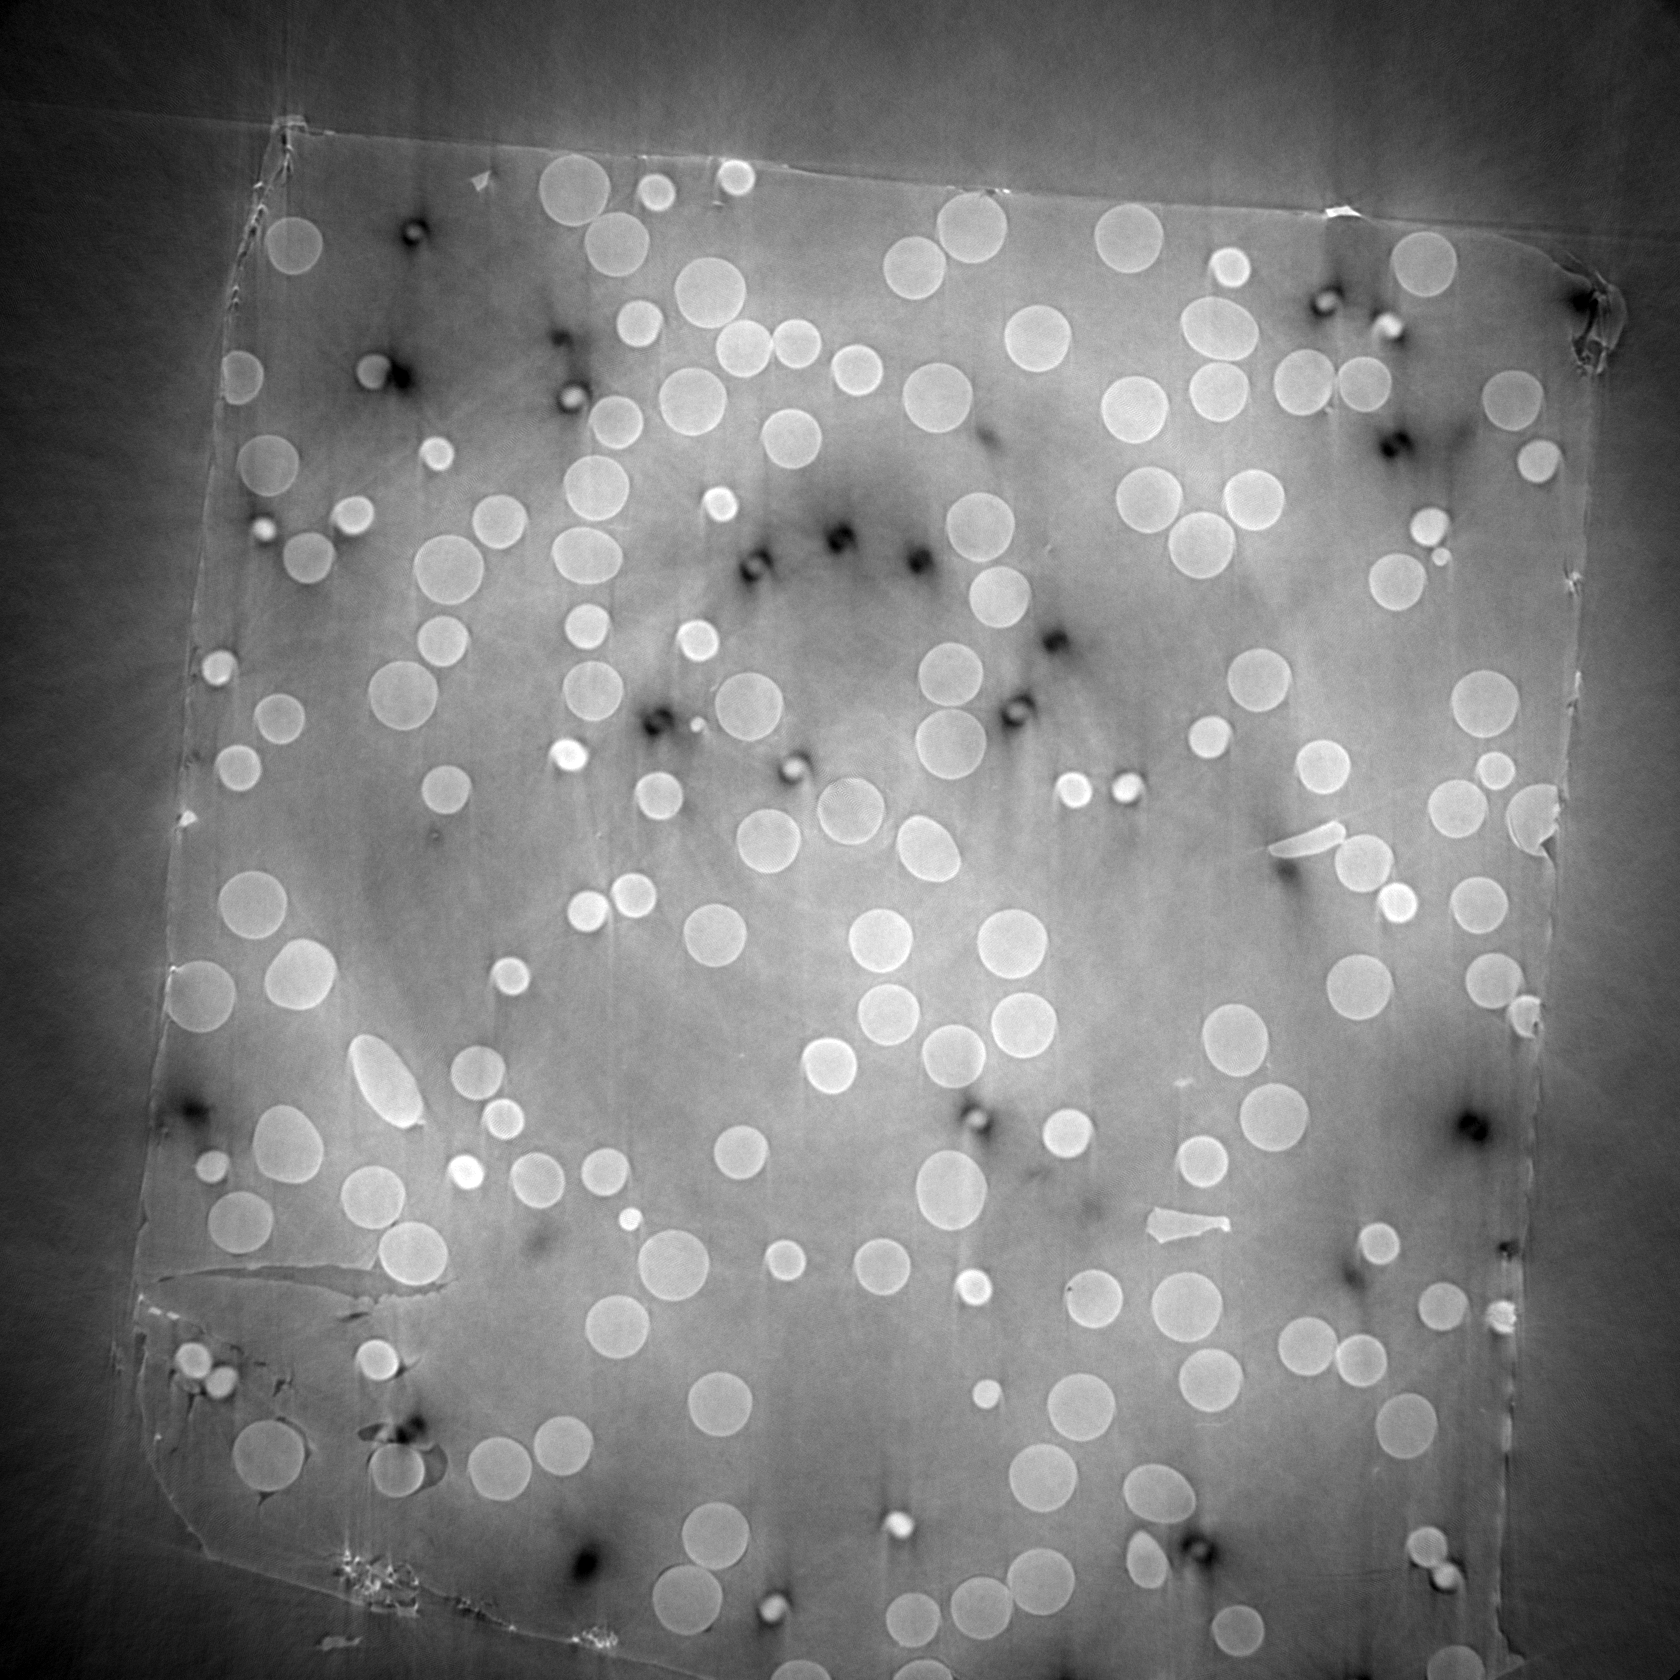
\includegraphics[width=.45\textwidth]{figures/gt32.png}
    \caption{\Gls{hq} (1500 projections). }
  \end{subfigure}

  \medskip

  \begin{subfigure}[t]{.45\textwidth}
    \centering
    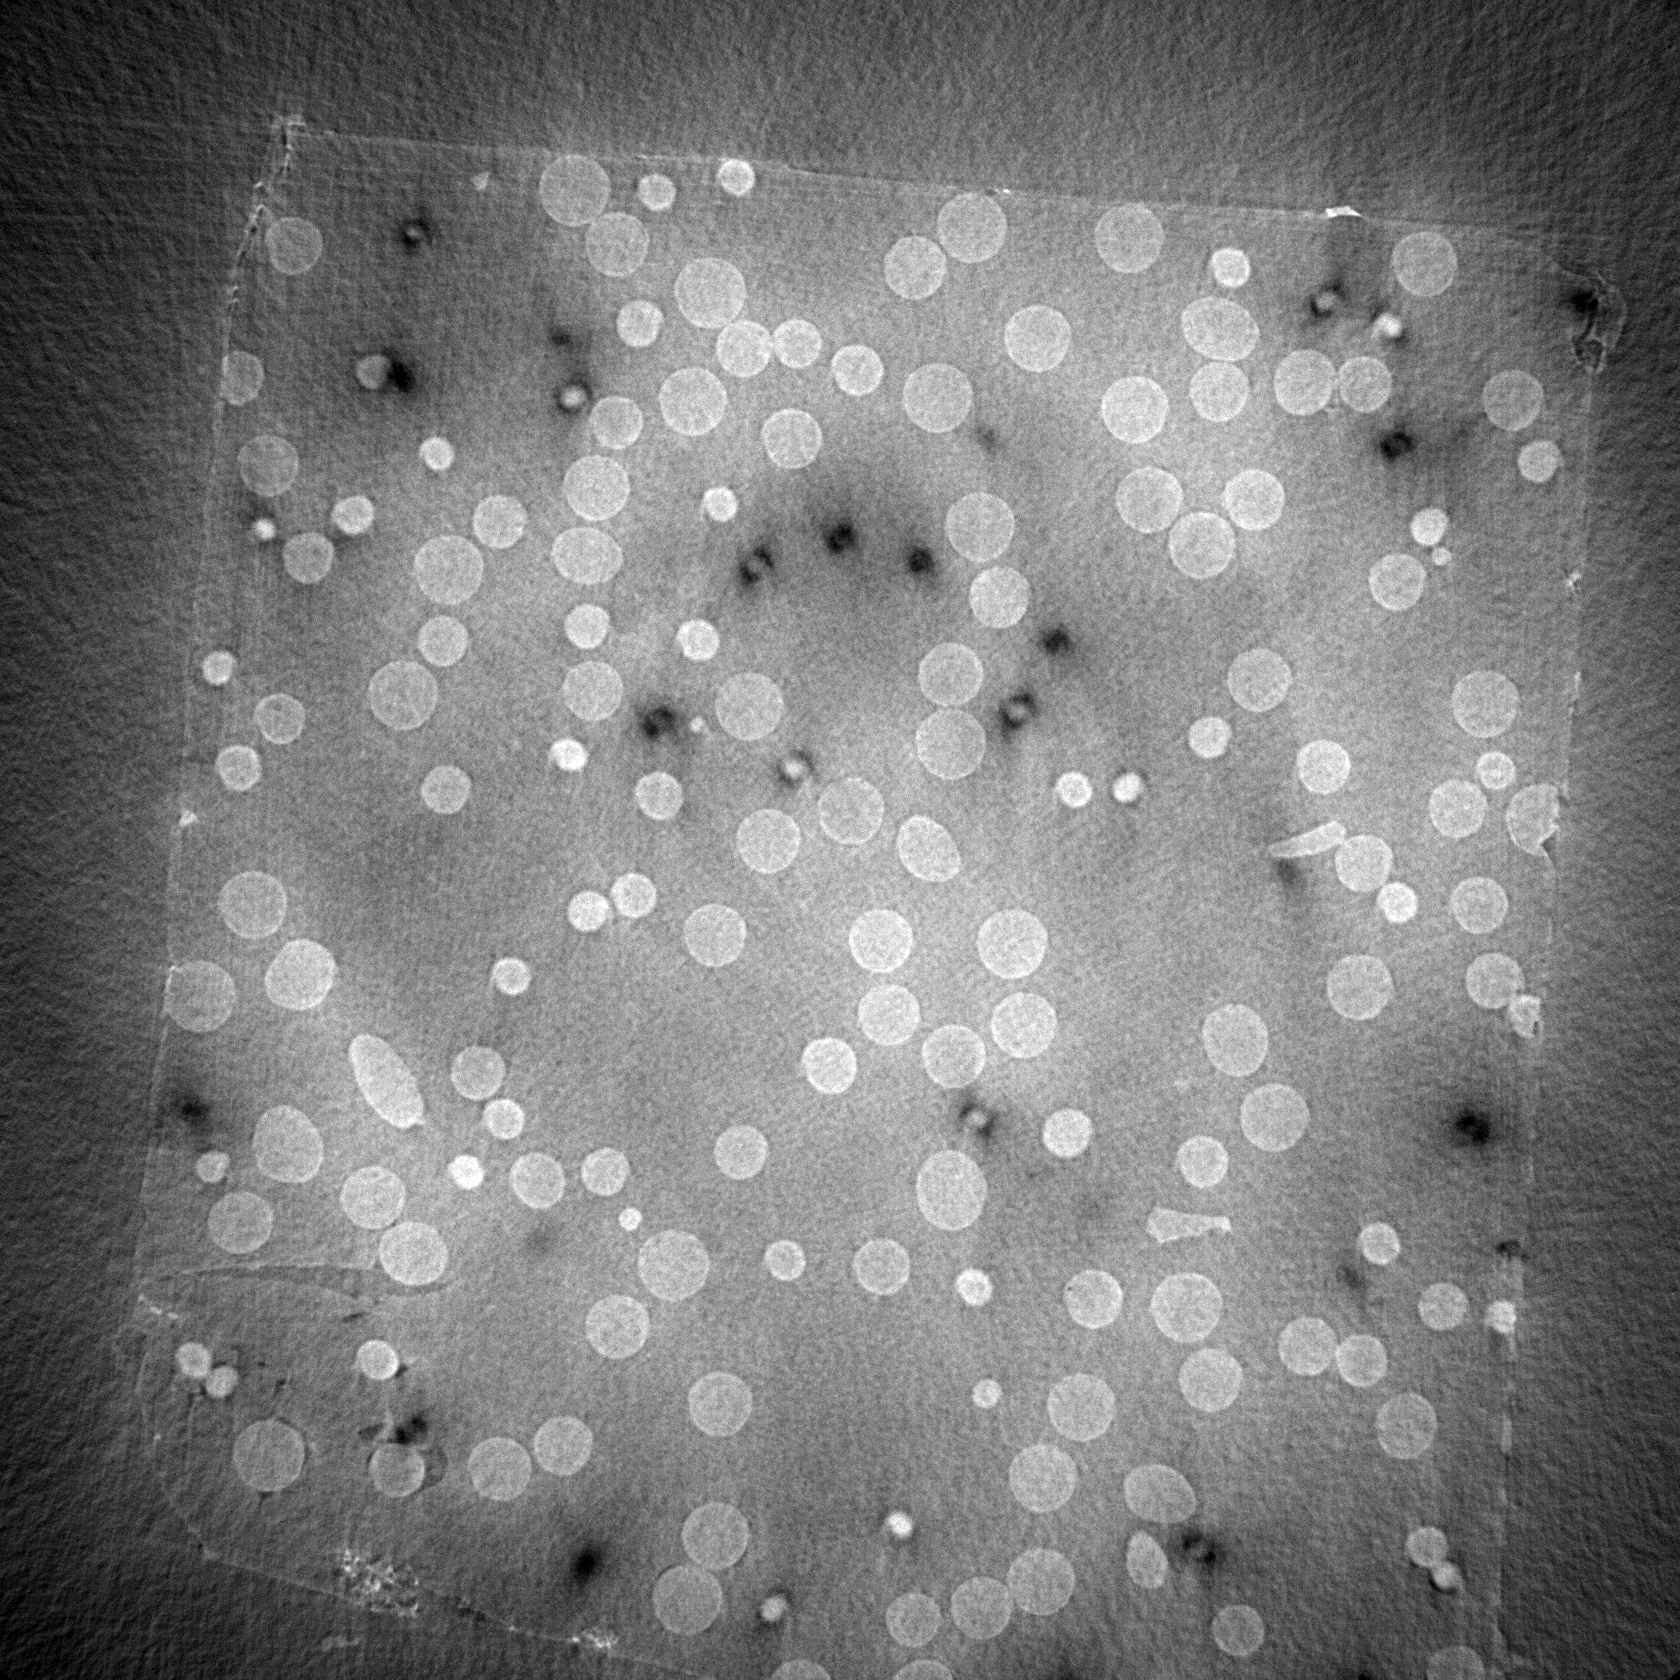
\includegraphics[width=\linewidth]{figures/ns8.png}
    \caption{Subsampling factor 8 (187 projections). }
  \end{subfigure}
  \hfill
  \begin{subfigure}[t]{.45\textwidth}
    \centering
    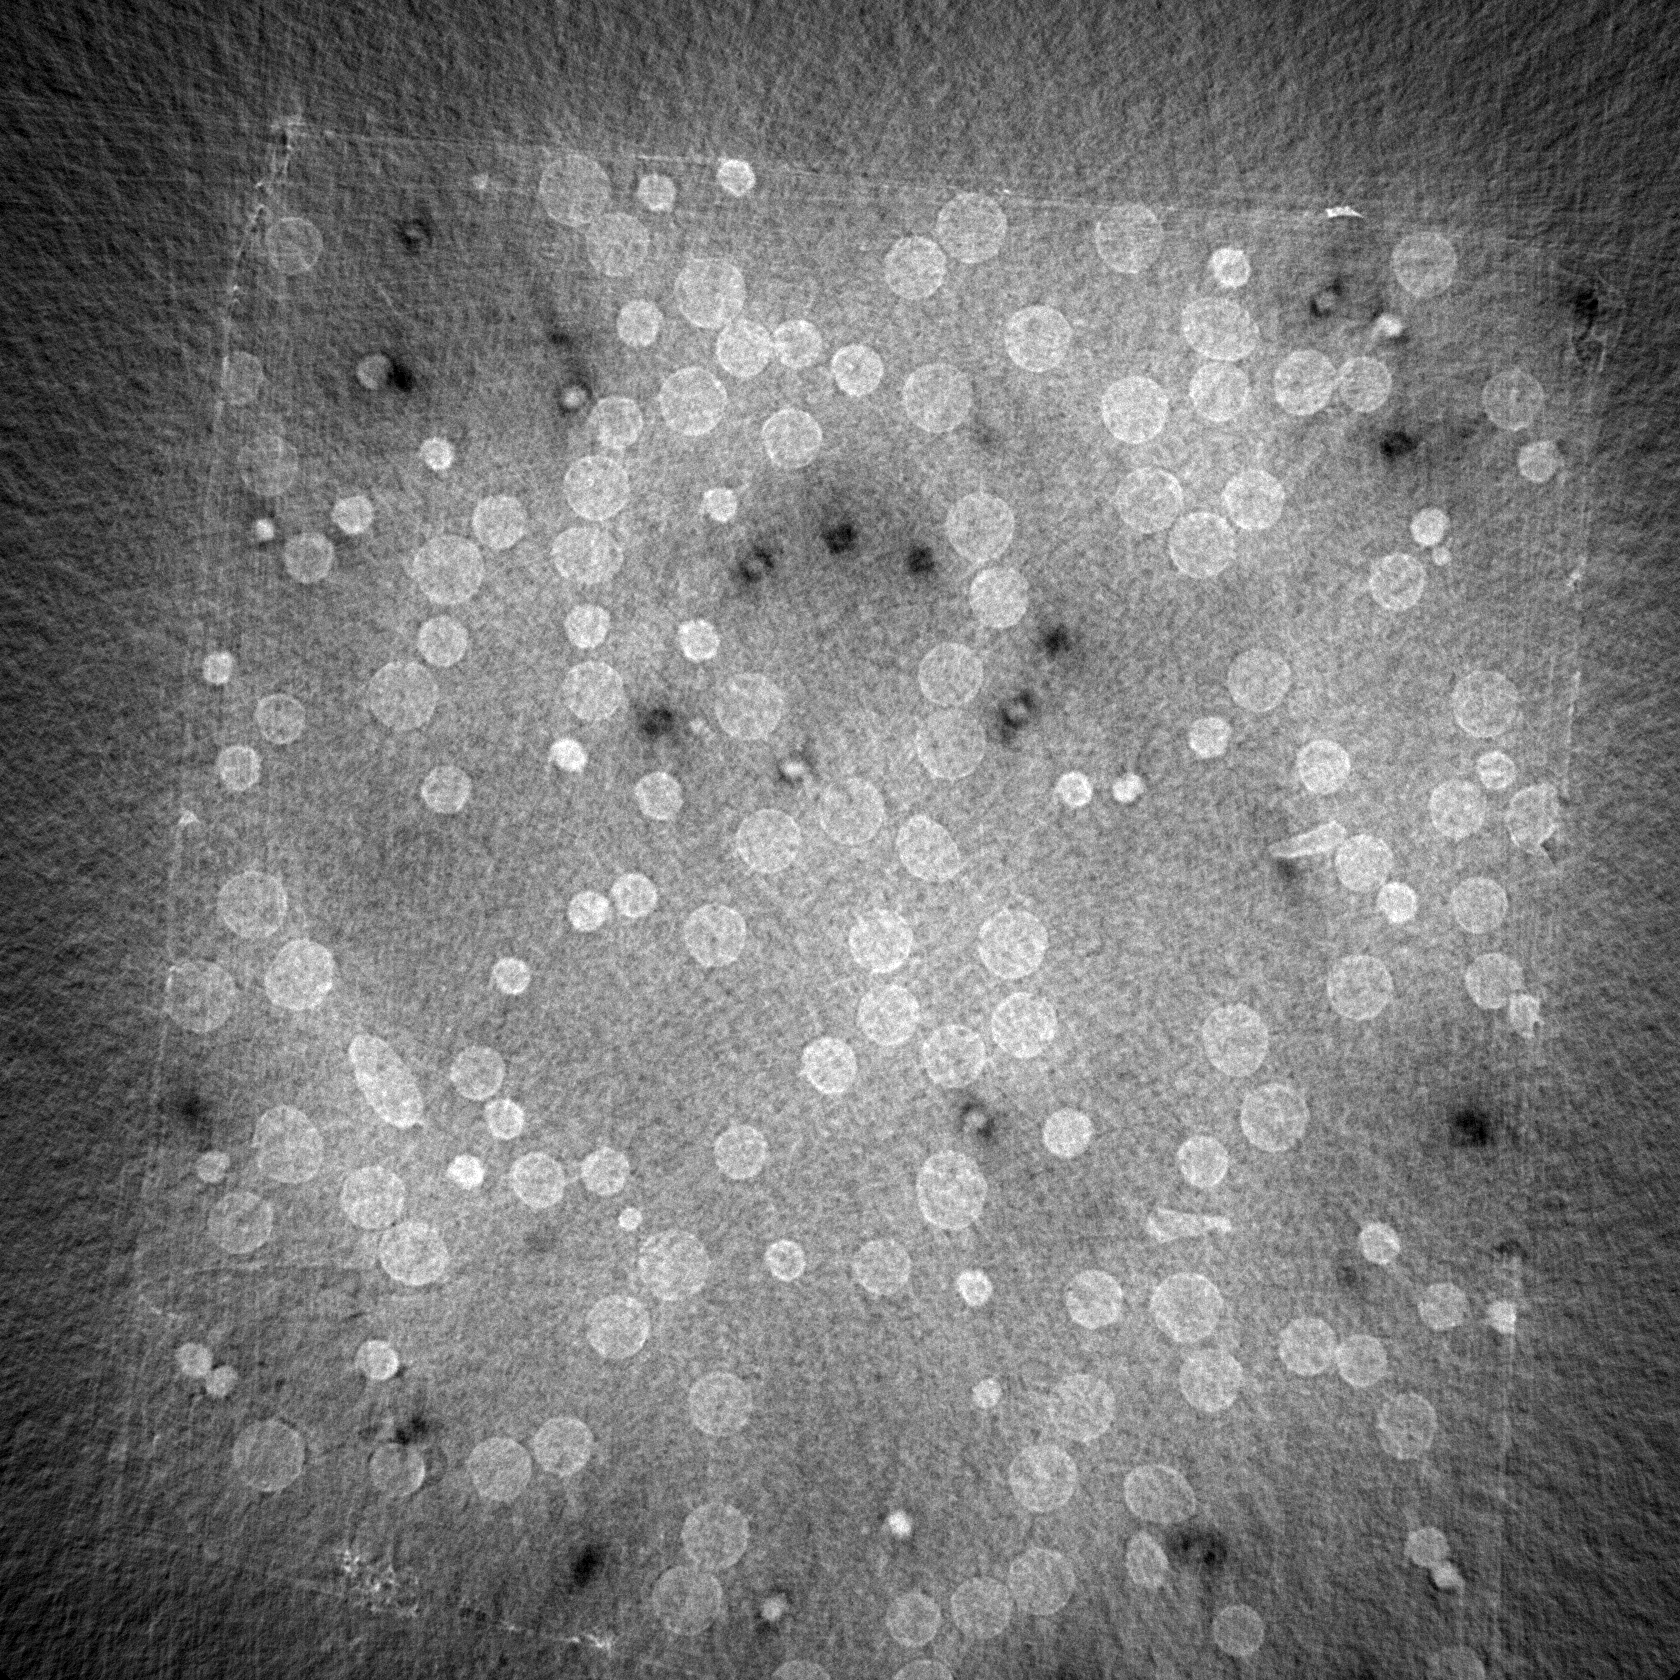
\includegraphics[width=\linewidth]{figures/ns16.png}
    \caption{Subsampling factor 16 (93 projections). }
  \end{subfigure}

  \medskip

  \begin{subfigure}[t]{.45\textwidth}
    \centering
    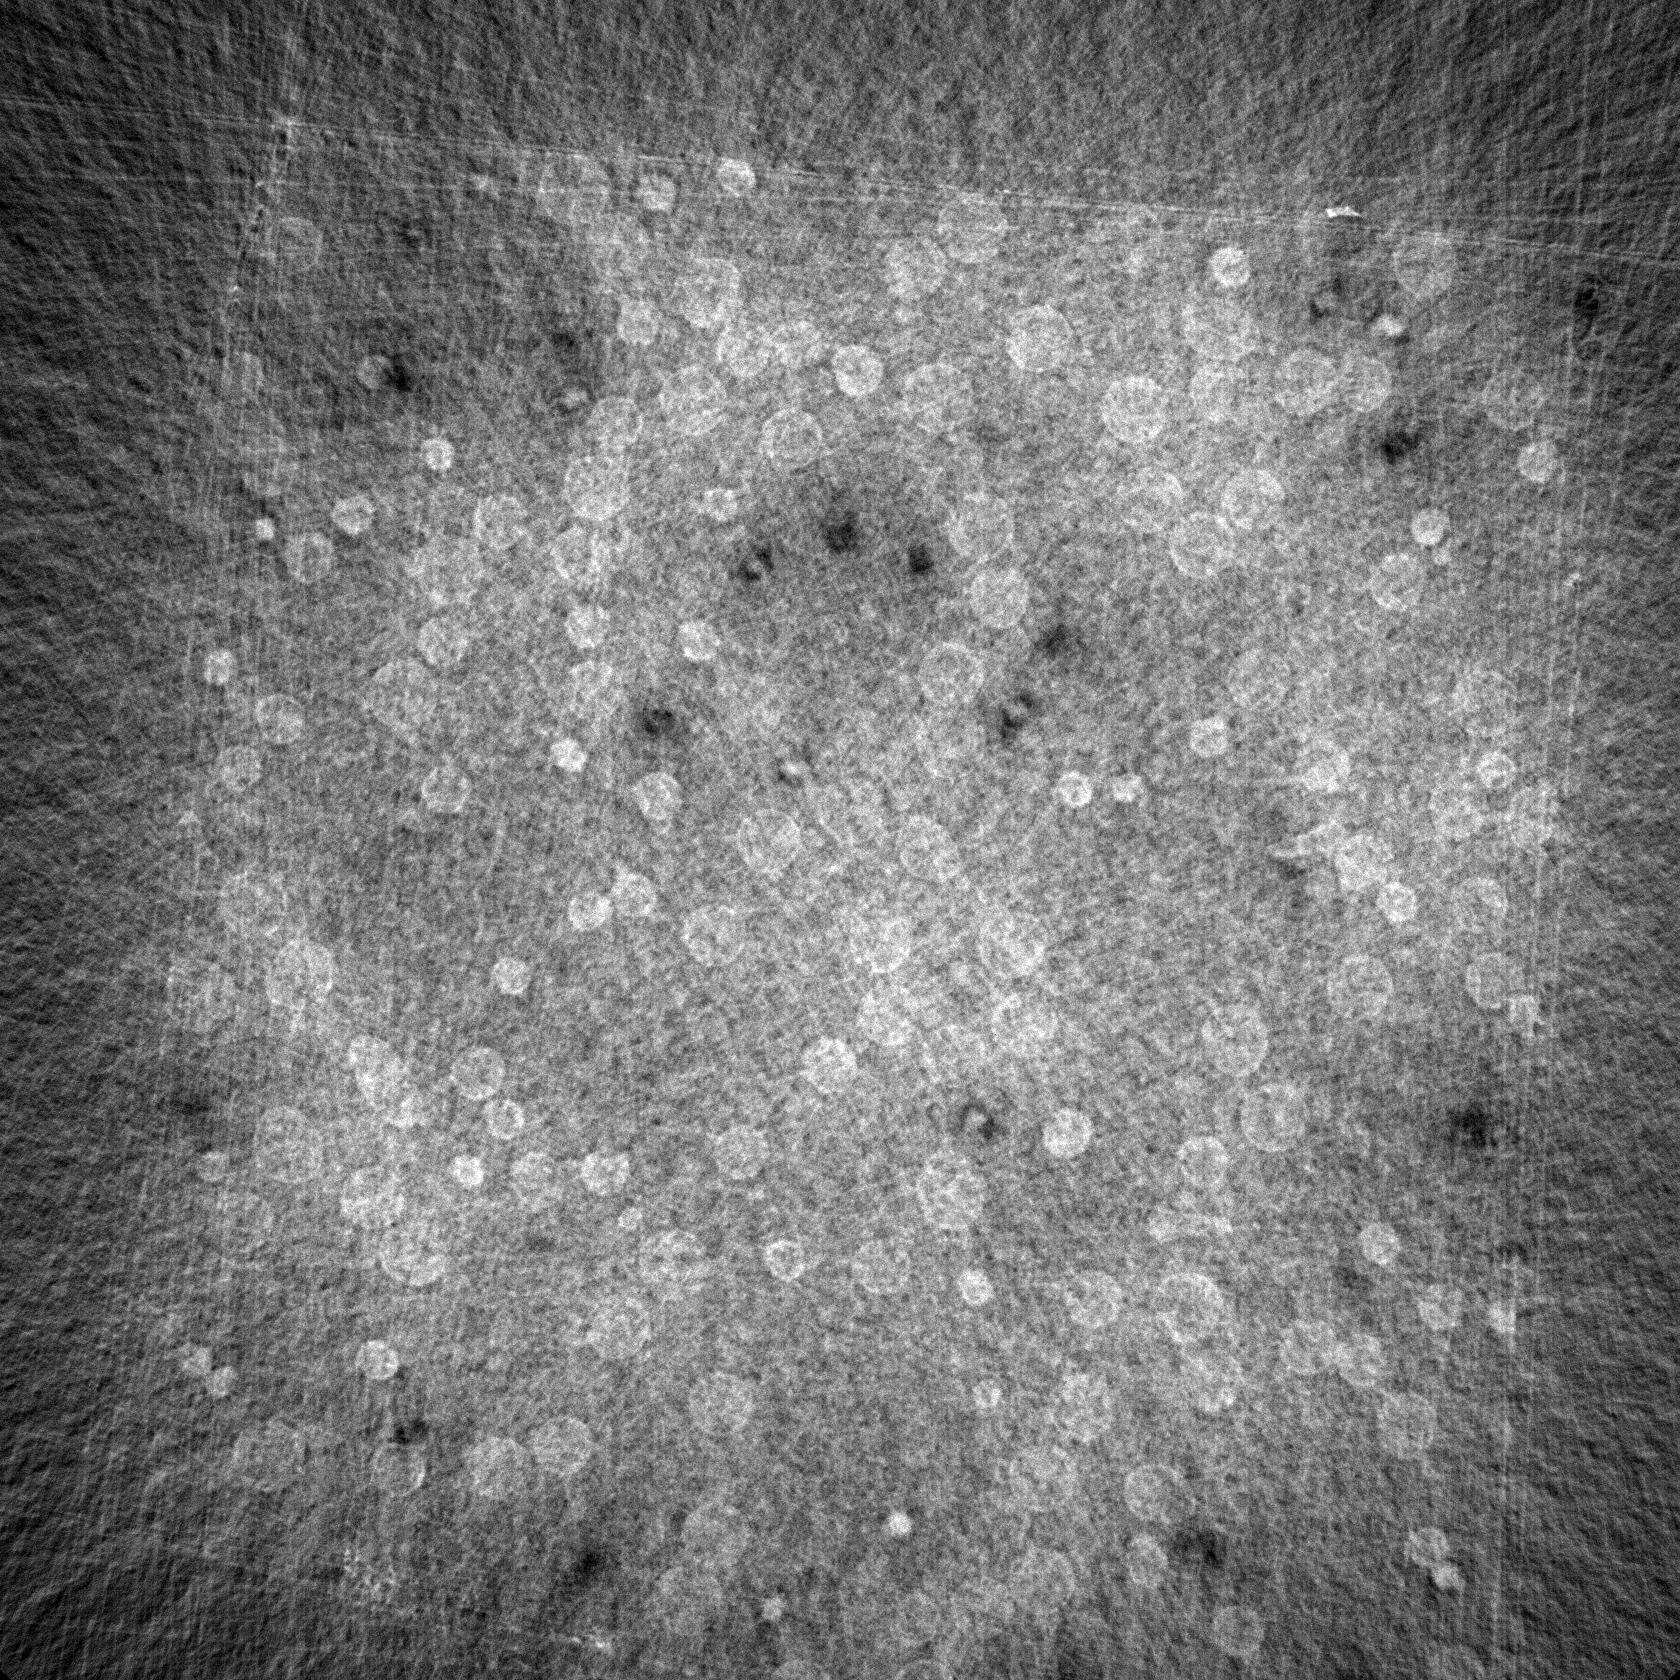
\includegraphics[width=\linewidth]{figures/ns32.png}
    \caption{Subsampling factor 32 (46 projections). }
  \end{subfigure}
  \hfill
  \begin{subfigure}[t]{.45\textwidth}
    \centering
    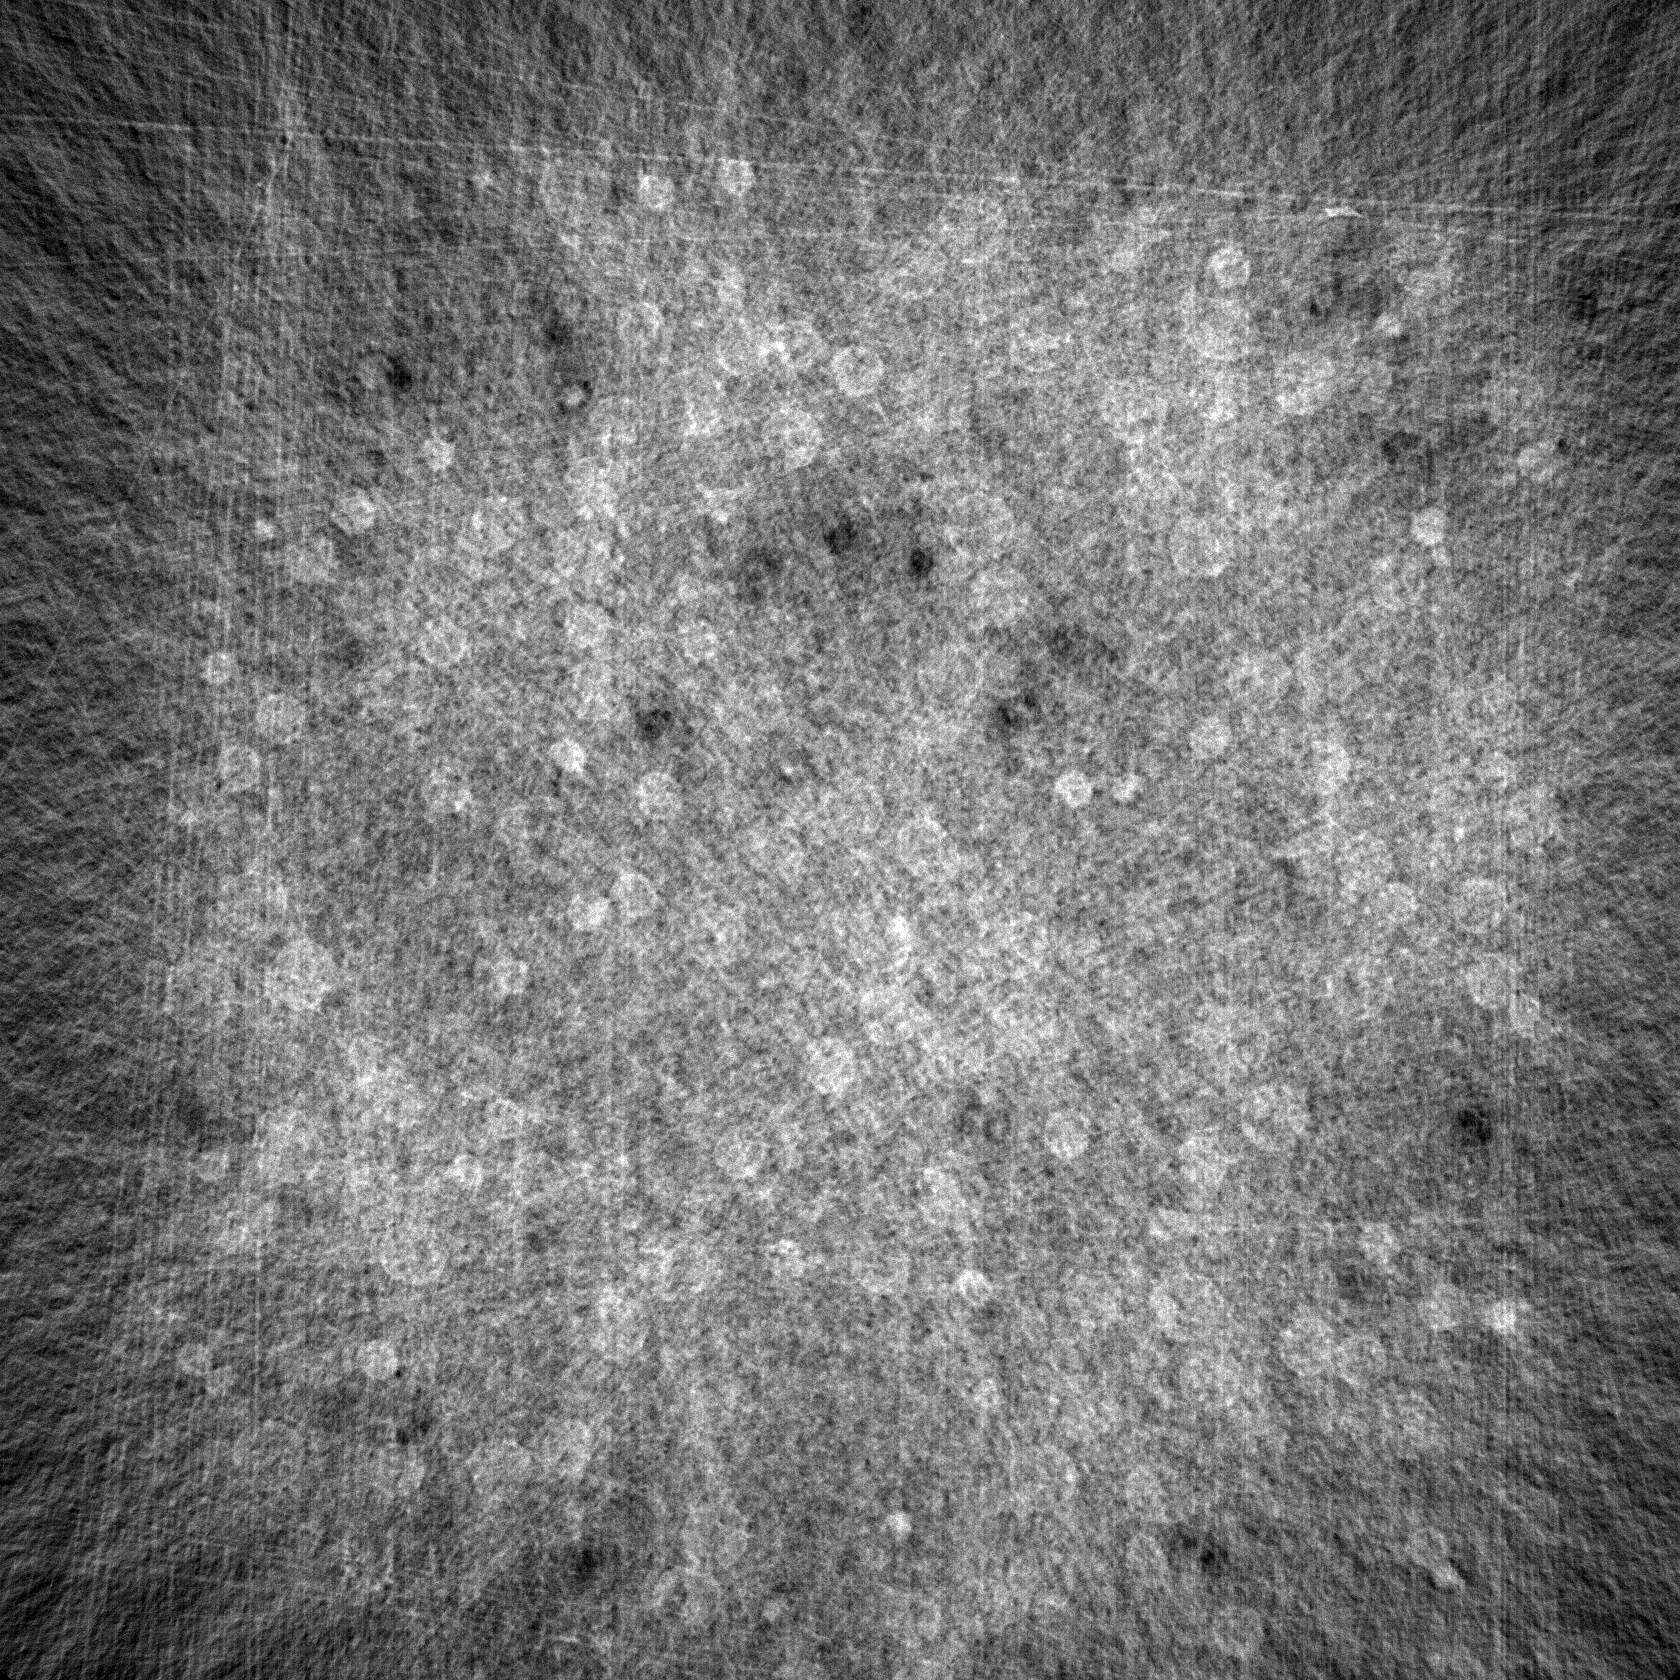
\includegraphics[width=\linewidth]{figures/ns48.png}
    \caption{Subsampling factor 48 (31 projections). }
  \end{subfigure}
  \caption[Four different levels of projection undersampling]{Comparison of different levels of projection undersampling on the borosilicate glass spheres dataset by reconstructing the images with the \gls{fbp} algorithm. The same cross-section is displayed for different reconstructions made by varying the number of projections used.  }
  \label{fig:tomo00058missingwedgecomparison}
\end{figure}

\begin{figure}
  \begin{subfigure}[t]{.45\textwidth}
    \centering
    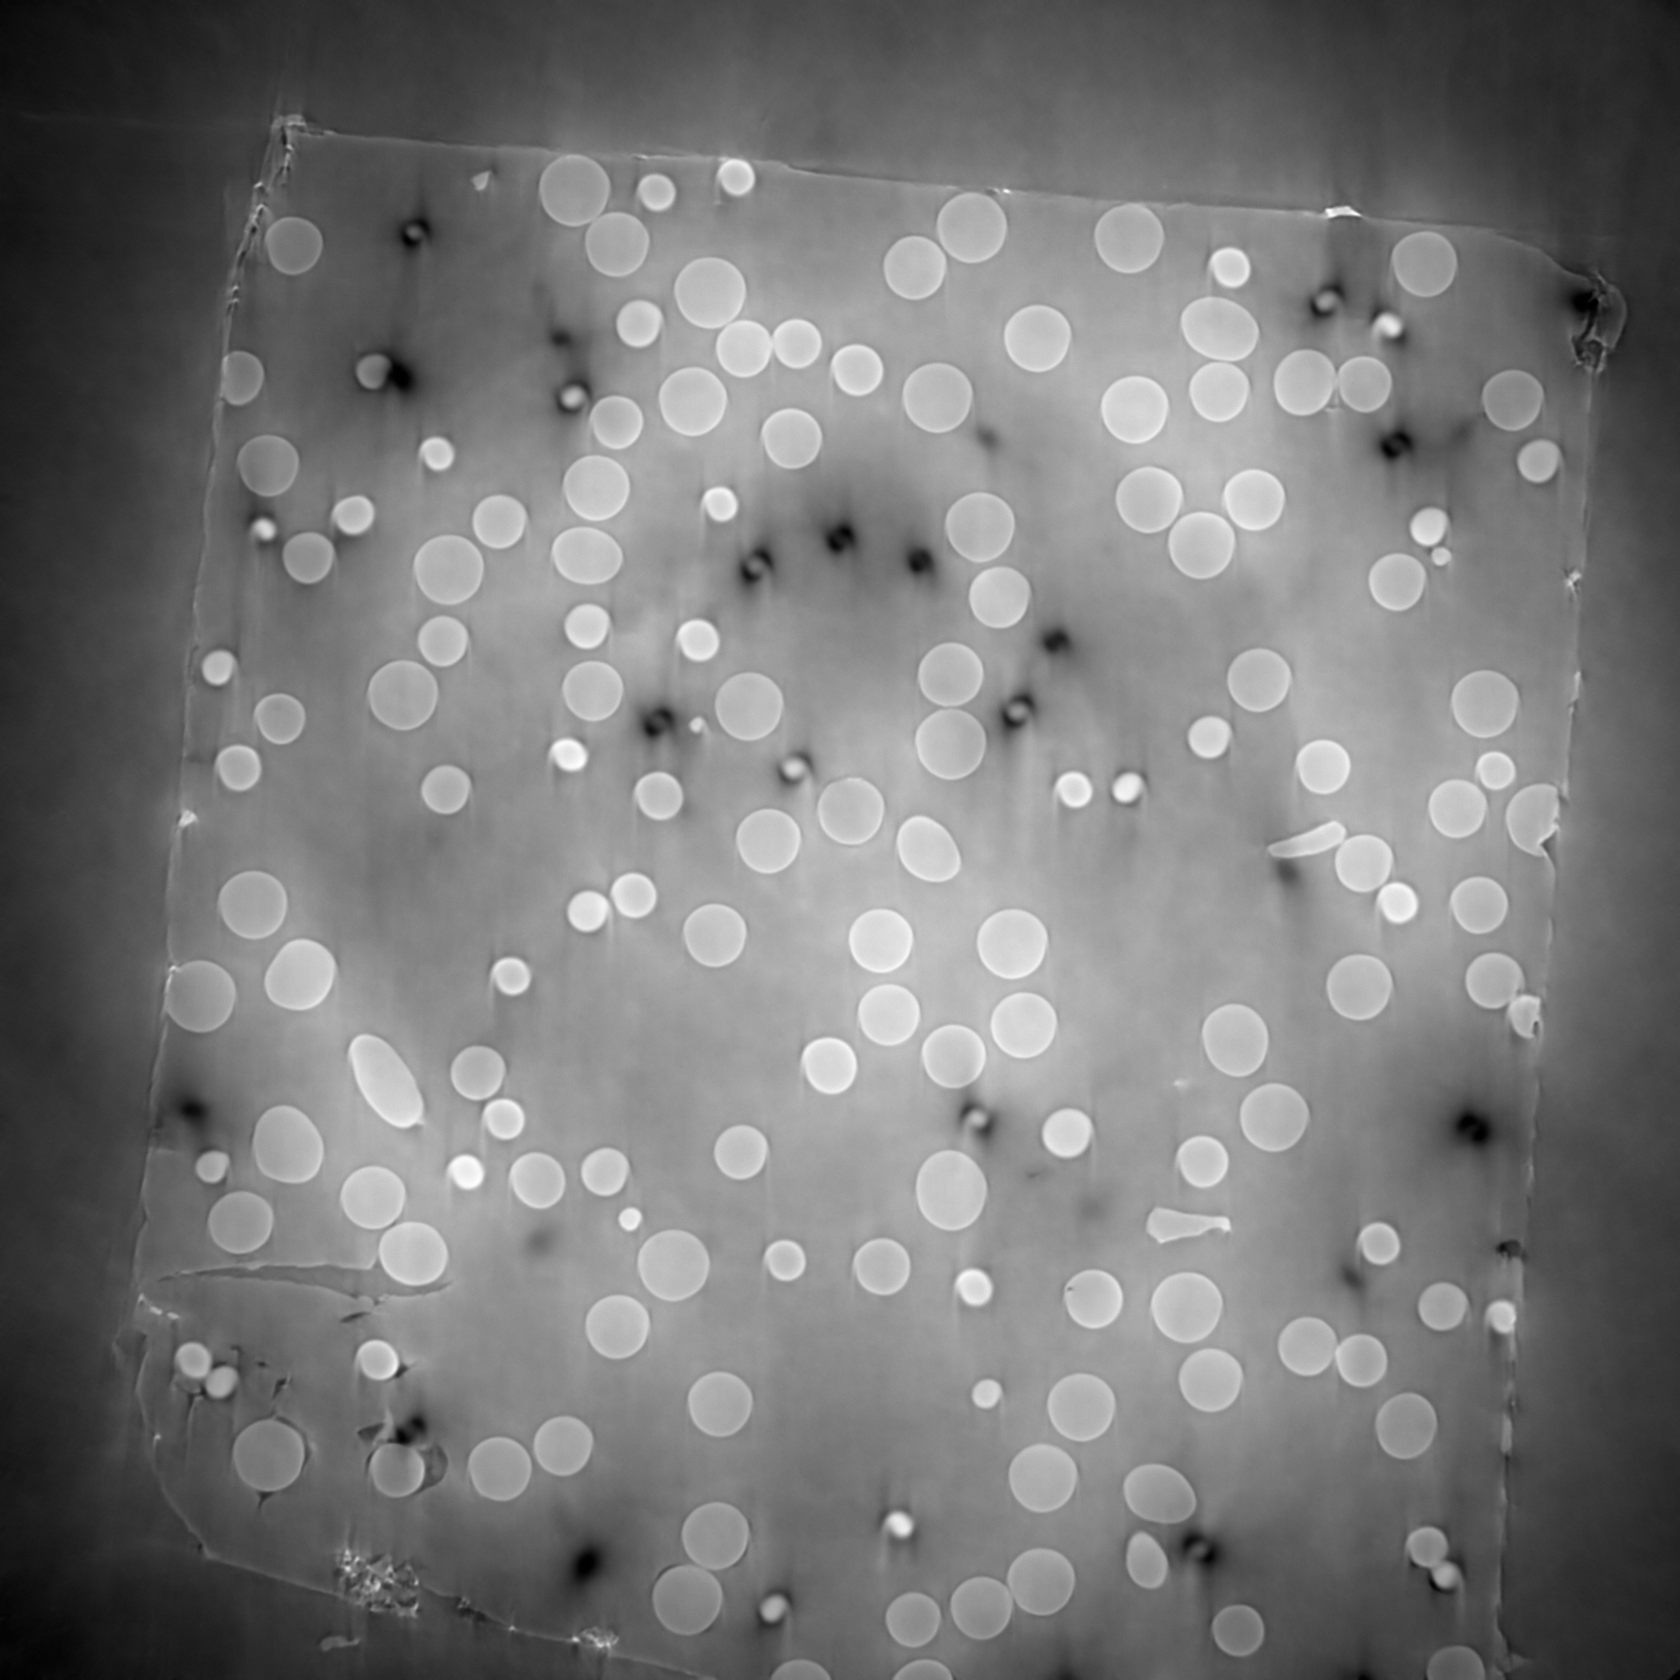
\includegraphics[width=\linewidth]{figures/ns8it100000itd4mse035logcosh3.png}
    \caption{Subsampling factor 8 (187 projections). }
  \end{subfigure}
  \hfill
  \begin{subfigure}[t]{.45\textwidth}
    \centering
    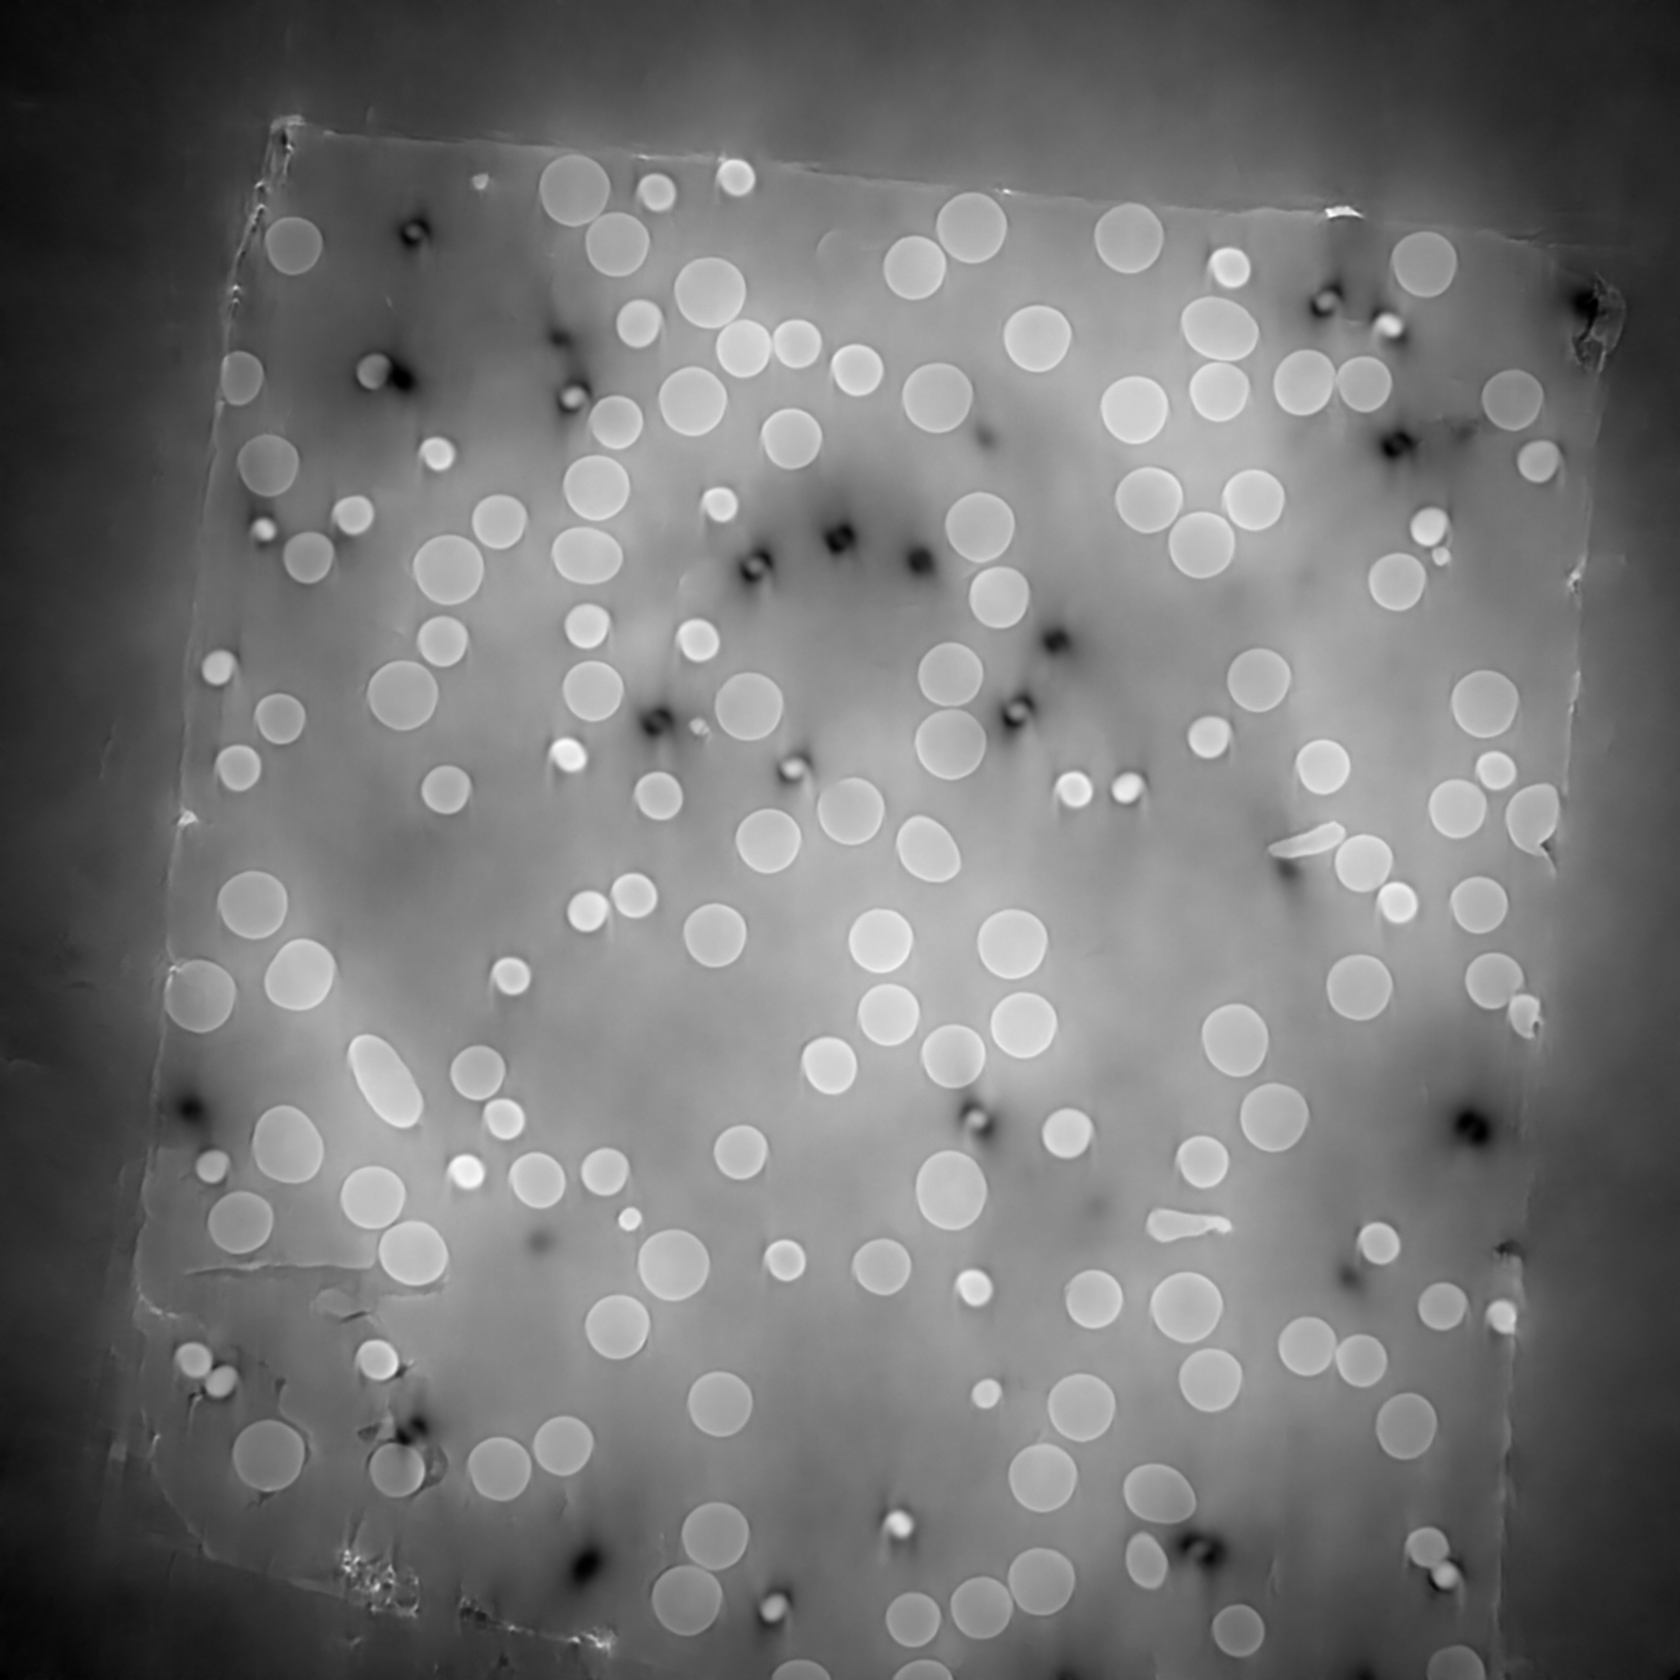
\includegraphics[width=\linewidth]{figures/ns16it100000itd4mse035logcosh3.png}
    \caption{Subsampling factor 16 (93 projections). }
  \end{subfigure}

  \medskip

  \begin{subfigure}[t]{.45\textwidth}
    \centering
    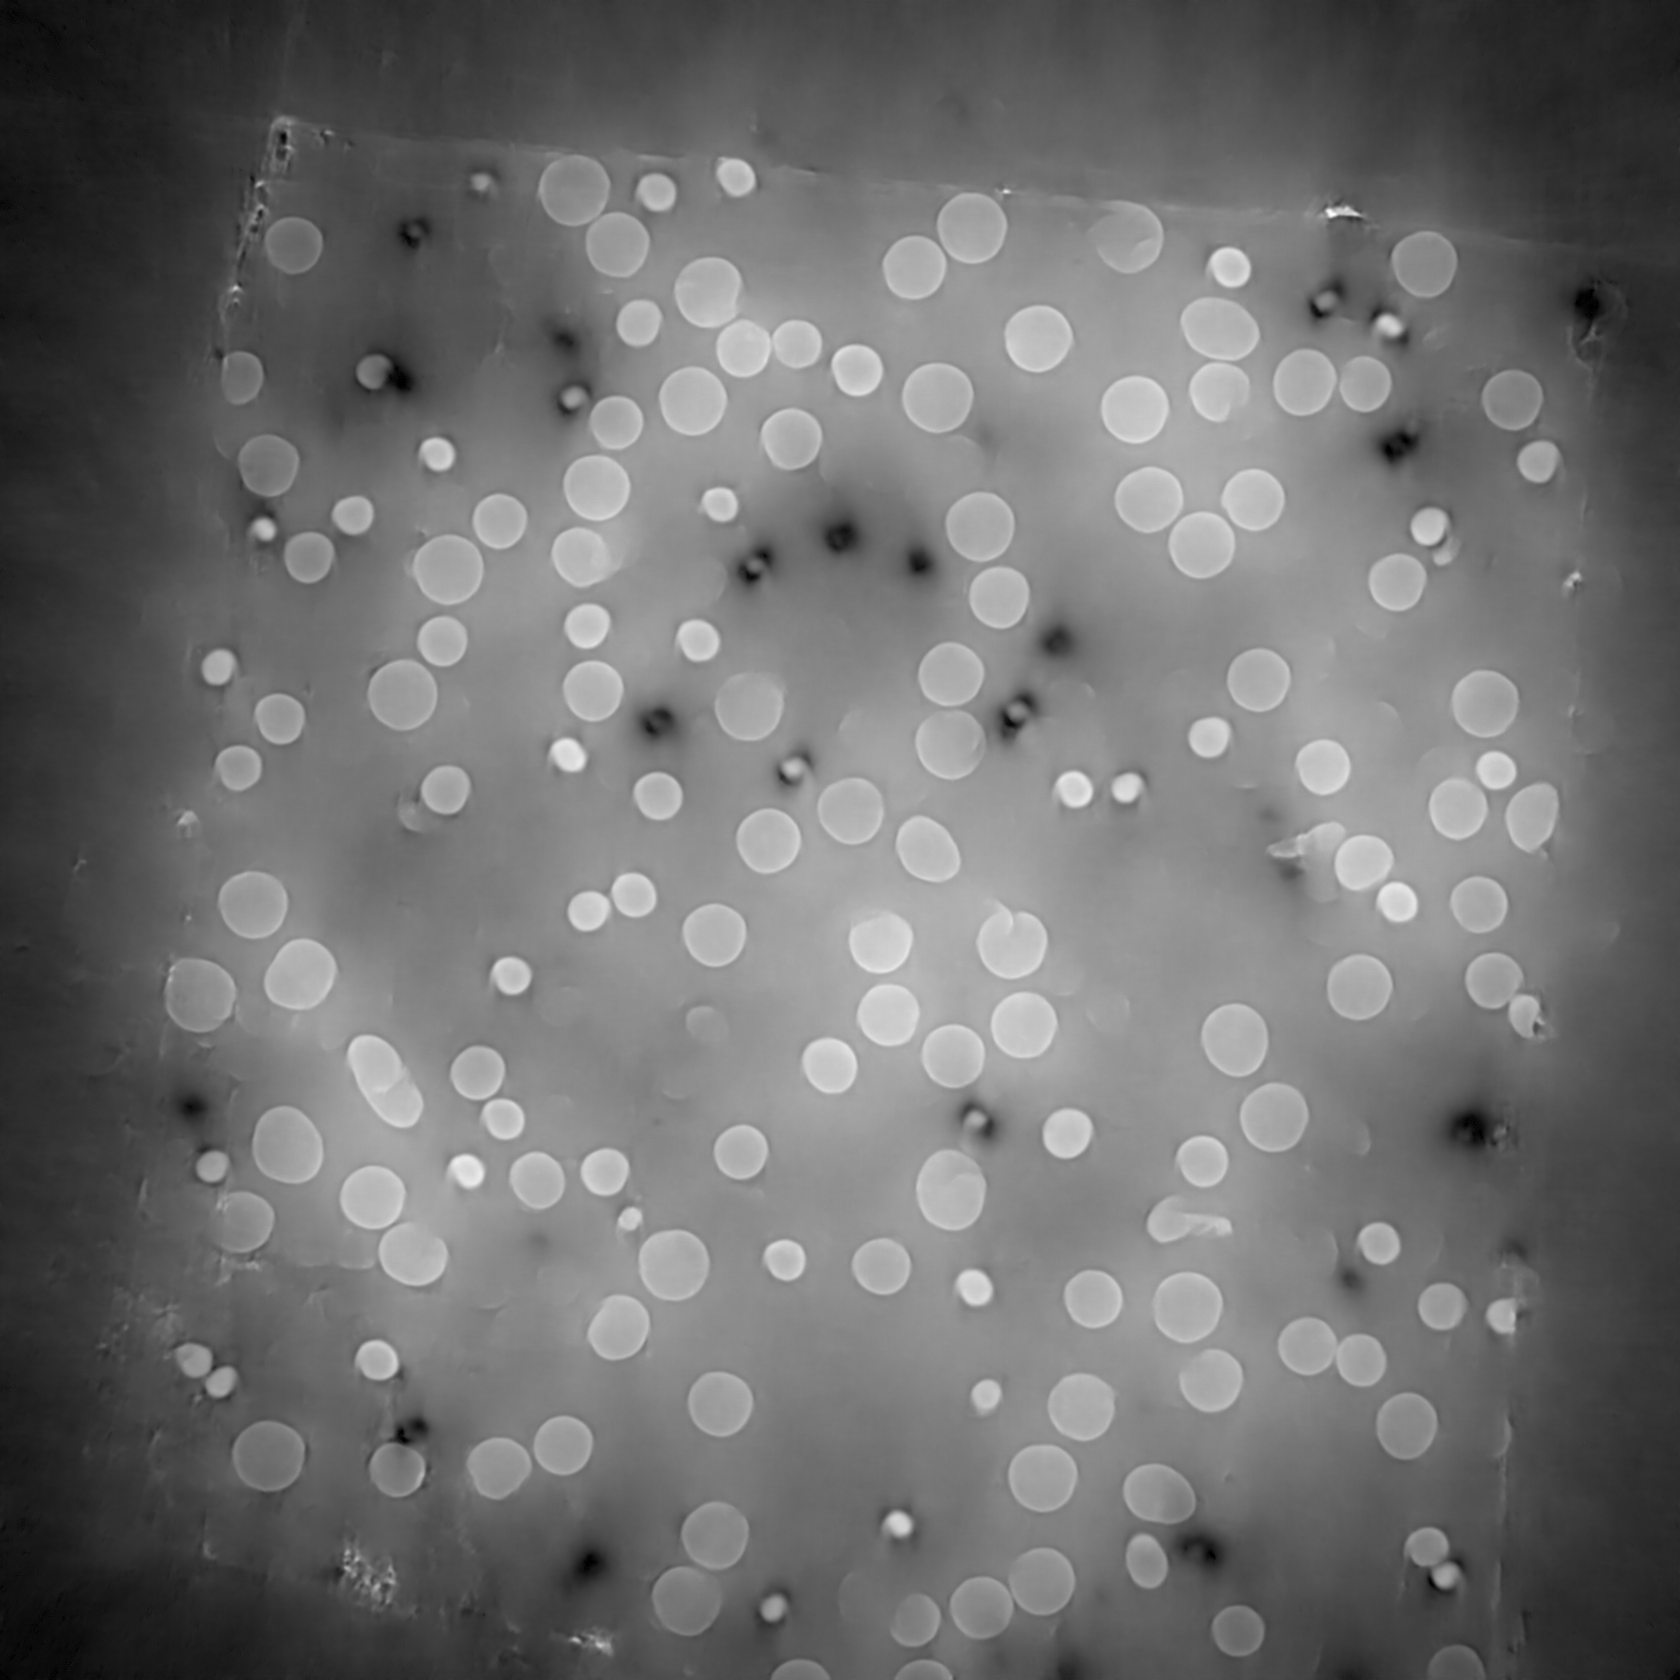
\includegraphics[width=\linewidth]{figures/ns32it100000itd4mse035logcosh3.png}
    \caption{Subsampling factor 32 (46 projections). }
  \end{subfigure}
  \hfill
  \begin{subfigure}[t]{.45\textwidth}
    \centering
    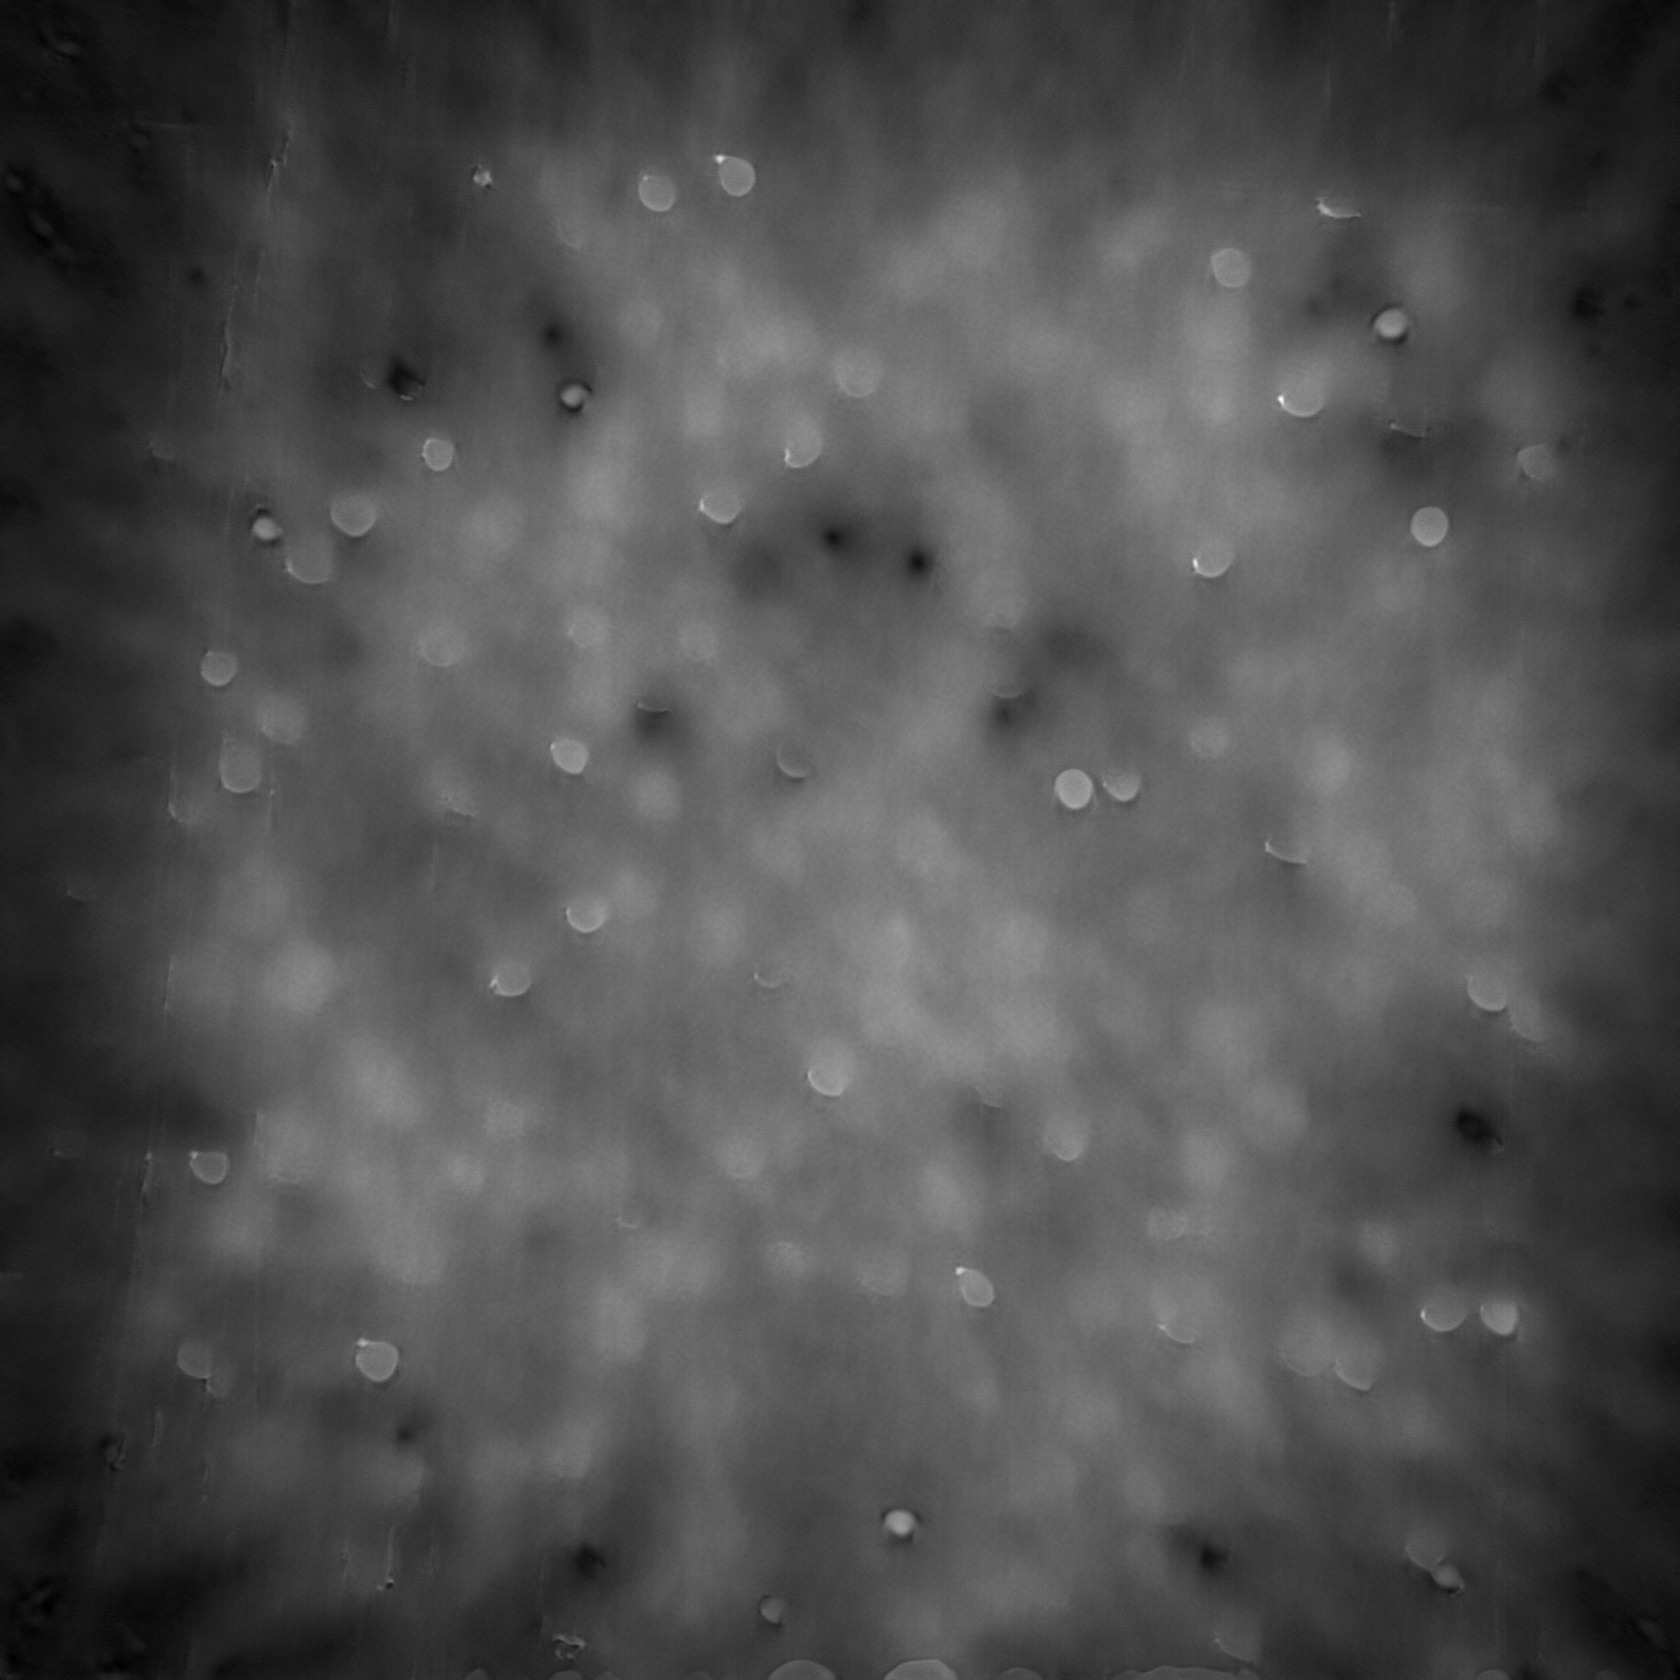
\includegraphics[width=\linewidth]{figures/ns48it100000itd4mse035logcosh3.png}
    \caption{Subsampling factor 48 (31 projections). }
  \end{subfigure}
  \caption[Denoising of four different levels of projection undersampling]{Comparison of denoising of different levels of projection undersampling on the borosilicate glass spheres dataset, where the corresponding noisy images are given in \cref{fig:tomo00058missingwedgecomparison}. The denoising was done with TomoGAN using a loss function containing \gls{mse}, log-cosh, VGG, and adversarial loss components, a depth of 1, and the network was trained for $100 000$ iterations with a mini batch size of 16. }
  \label{fig:tomo00058missingwedgecomparisondenoised}
\end{figure}

It is evident that a subsampling factor of 48, corresponding to merely 31 projections, leads to too much noise to recover any usable denoised image. This is further confirmed by looking at plots of the pixel values along two different lines on the denoised images and comparing them with the noisy and the \gls{hq} image, as can be seen in \cref{fig:differentnoiselineplot1,fig:differentnoiselineplot2}. For the other three datasets the denoising seems to result in images sufficiently similar to the \gls{hq} image, especially for subsampling factors $8$ and $16$. 

\begin{figure}[htbp]
  \centering
  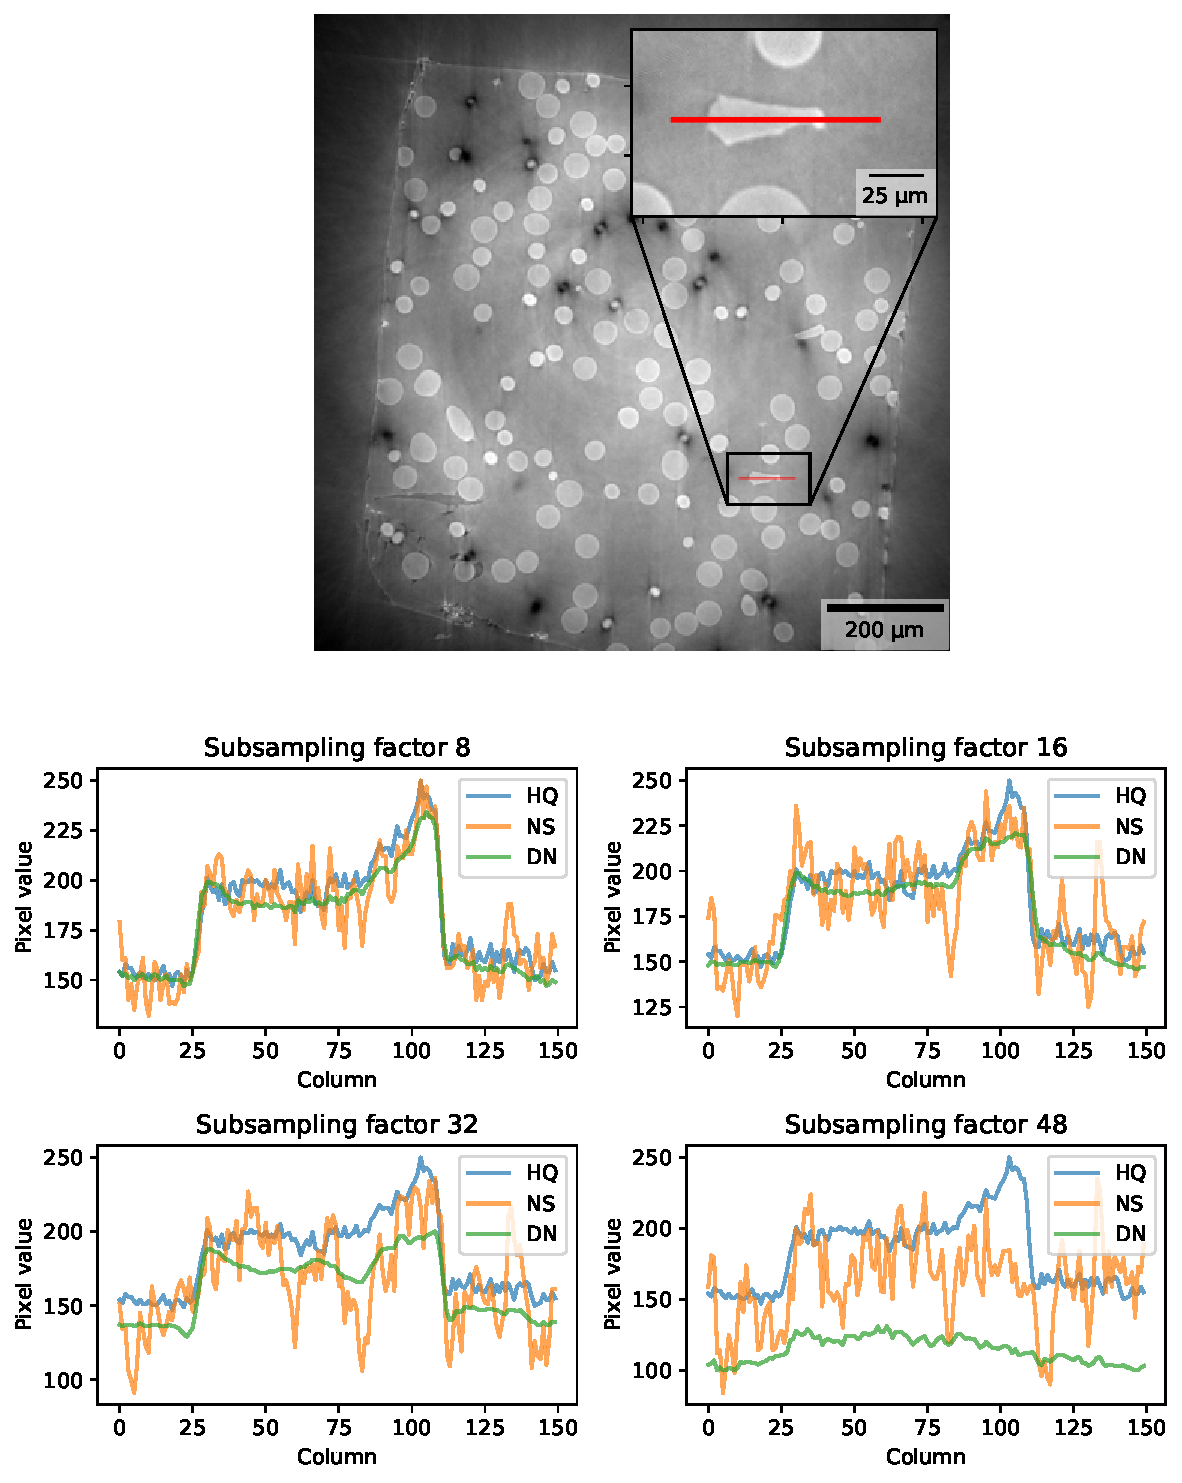
\includegraphics[width=.95\textwidth]{figures/differentnoiselineplot1.pdf}
  \caption[Pixel value plot of denoising of different levels of projection undersampling on the borosilicate glass spheres dataset]{The plots show pixel values for 150 pixels on a horizontal line on the borosilicate glass spheres dataset, as shown by the red line on the \gls{hq} image above, for denoising of four different levels of projection undersampling. \gls{hq} corresponds to the \gls{hq} image, NS to the \gls{lq} image, and \gls{dn} to the denoised image. All denoising was done with TomoGAN using a loss function containing \gls{mse}, log-cosh, VGG, and adversarial loss components, a depth of 1, and the network was trained for $100 000$ iterations with a mini batch size of 16. }
  \label{fig:differentnoiselineplot1}
\end{figure}

\begin{figure}[htbp]
  \centering
  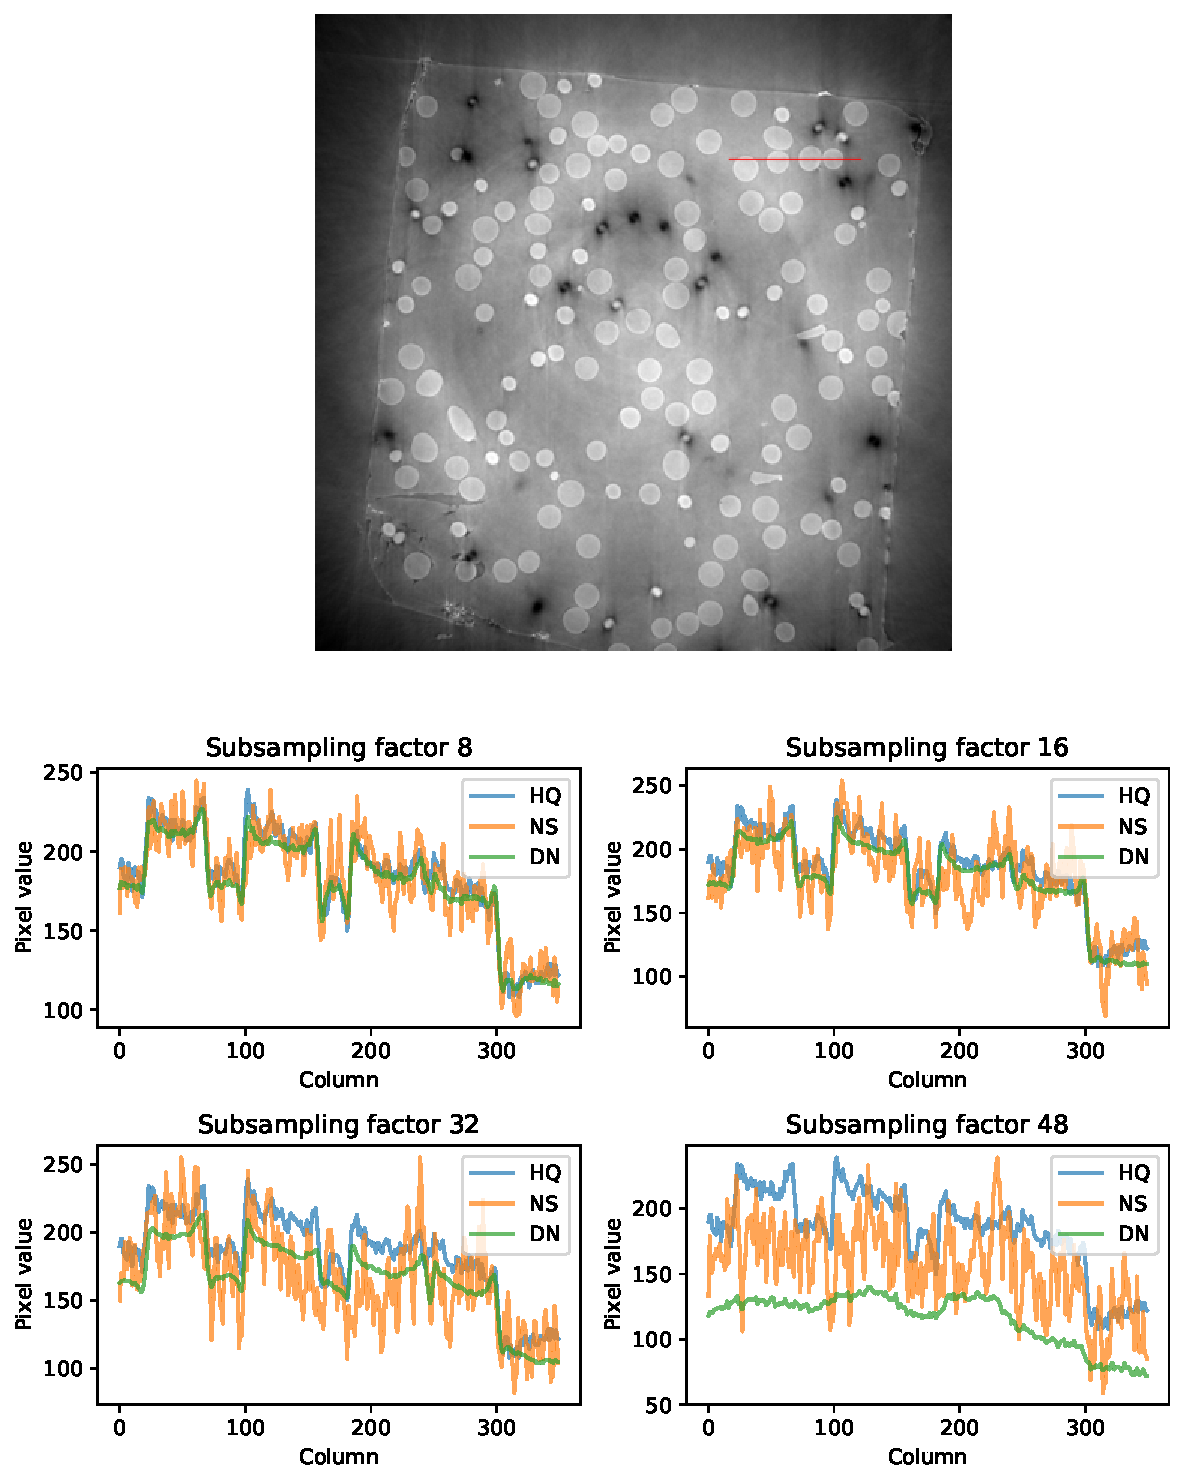
\includegraphics[width=.95\textwidth]{figures/differentnoiselineplot2.pdf}
  \caption[Pixel value plot of denoising of different levels of projection undersampling on the borosilicate glass spheres dataset]{The plots show pixel values for 400 pixels on a horizontal line on the borosilicate glass spheres dataset, as shown by the red line on the \gls{hq} image above, for denoising of four different levels of projection undersampling. Figure elements are as in \cref{fig:differentnoiselineplot1}. }
  \label{fig:differentnoiselineplot2}
\end{figure}

\cref{tab:missingwedgessim} contains \gls{ssim} and \gls{mse} values for the noisy and denoised images shown in \cref{fig:tomo00058missingwedgecomparison,fig:tomo00058missingwedgecomparisondenoised}. We see here that for subsampling factors $8$, $16$, and $32$, the \gls{mse} is improved by denoising, however for subsampling factor $48$ it is drastically worsened. All denoisings achieve, to varying degrees, \gls{ssim} improvements. The fact that the poor denoising of the subsampling factor of $48$ achieves an improvement in \gls{ssim} from $0.193$ to $0.657$ indicates that \gls{ssim} is not able to sufficiently gauge the image quality in this case. 

It is worth noting that a subsampling factor of $32$ corresponds to $46$ projections, which is similar to the $64$ projections used in the noisiest simulated dataset in the original article by Liu \textit{et al.} \cite{liu2020tomogan}. The achieved \gls{ssim} score on a real dataset of $0.789$ in this thesis is similar to their results on a simulated phantom. 

\begin{table}[htbp]
  \centering
  \caption[SSIM for different levels of simulated projection undersampling and corresponding values after denoising]{Overview of \gls{ssim} for different levels of simulated projection undersampling on the borosilicate glass spheres dataset. The projection undersampling was simulated by subsampling the number of projections by a factor as given in the subsampling factor column. All denoising was done with TomoGAN using a loss function containing \gls{mse}, log-cosh, VGG, and adversarial loss components, a depth of 1, and the network was trained for $100 000$ iterations with a mini batch size of 16. }
  \label{tab:missingwedgessim}
  \begin{tabular}{llllll}
  \hline
  \multirow{2}{*}{Subsampling factor} & \multirow{2}{*}{Projections} & \multicolumn{2}{c}{\gls{ssim}} & \multicolumn{2}{c}{\gls{mse}}  \\
  {} & {} & Noisy & Denoised & Noisy & Denoised \\
  \hhline{======}
  %\hline 
  $1$  & $1500$ & $1.0$ & $-$ & $0.0$ & $-$ \\
  $8$  & $187$ & $0.492$ & $0.842$ & $148.3$ & $33.3$ \\
  $16$ & $93$ & $0.335$ & $0.816$ & $348.5$ & $74.9$ \\
  $32$ & $46$ & $0.233$ & $0.789$ & $704.4$ & $210.8$ \\
  $48$ & $31$ & $0.193$ & $0.657$ & $976.6$ & $2362.6$ \\
  \hline
  \end{tabular}
\end{table}

\subsection{Effect of Pre-processing Images}
Attempting to denoise the borosilicate glass spheres dataset without cropping the reconstructed images yielded poor results, as is given in \cref{fig:uncroppeddenoising}. The network does not seem to have managed to converge properly, and the results look to simply be bluring the images. The use of an \gls{mse} based loss function may be part of the cause of the blurring, as this loss has been shown to cause blurring in image processing related tasks such as this. 

When the images are all cropped, with no other changes being made, the network performs better. This is given in \cref{fig:croppeddenoising}. While there is artefacting from the denoising (especially when looking at shapes that differ from the common shapes in the dataset, such as non-circular shapes), when comparing the \gls{hq} and \gls{dn} images it is evident that a majority of the features have been preserved with the noise being drastically reduced. 

Comparing the non-cropped denoising with a denoising only run with a few iterations, not reaching full convergence, as seen in \cref{fig:croppednoncroppedearly}, the results are similar indicating that the non-cropped denoising may have struggled to converge properly. 

Note that the images in \cref{fig:uncroppeddenoising,fig:croppeddenoising} have different intensity scales because of the scaling step of the preprocessing (see \cref{sec:method:compilingdataset}). 

This denoising was performed with TomoGAN using a loss function containing \gls{mse}, log-cosh, VGG, and adversarial loss components, a depth of 1, and the network was trained for 100000 iterations with a mini batch size of 16 (see \cref{sec:ml}). 

\begin{figure}[htbp]
  \centering
  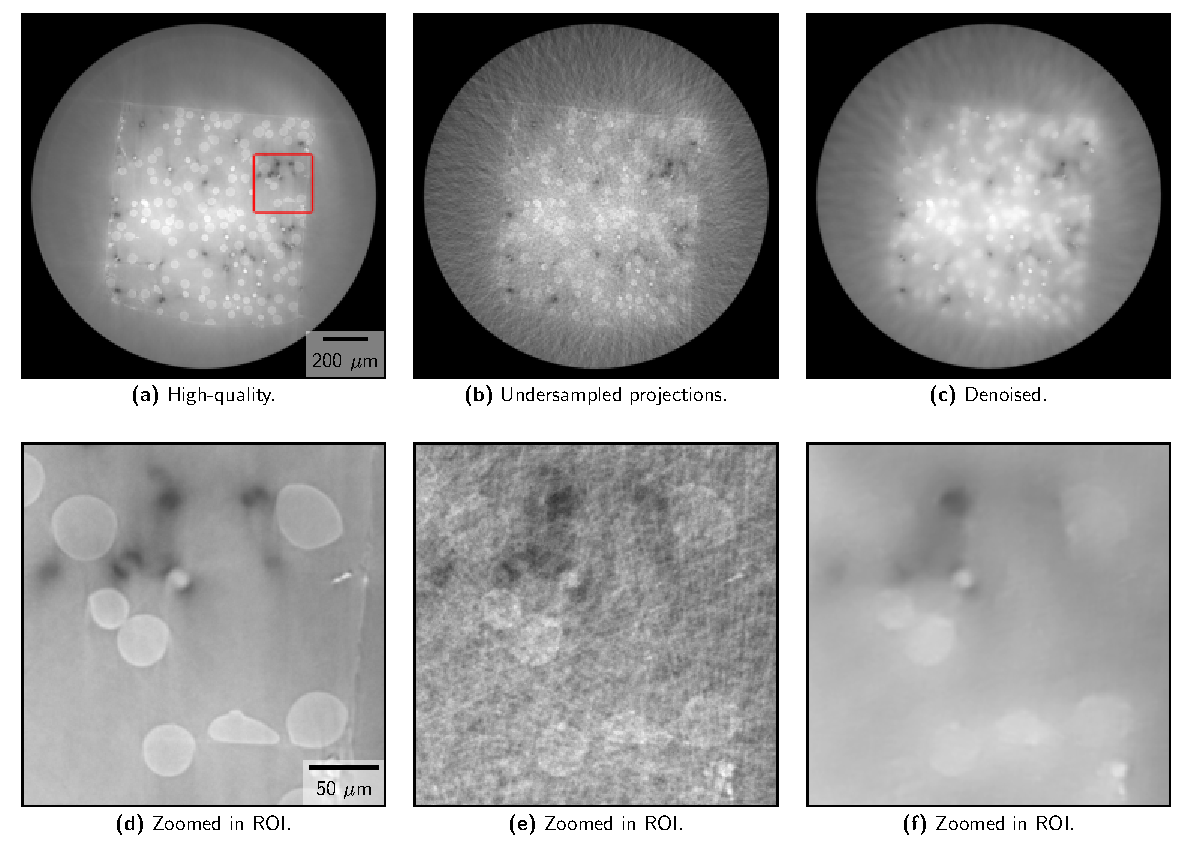
\includegraphics[width=.9\textwidth]{figures/uncroppeddenoising.pdf}
  \caption[Non-cropped image denoising]{Denoising of non-cropped borosilicate glass spheres dataset. Images d), e), and f) are zoomed in \gls{roi}s of images a), b), and c) respectively. The \gls{roi} is marked in a). }
  \label{fig:uncroppeddenoising}
\end{figure}

\begin{figure}[htbp]
  \centering
  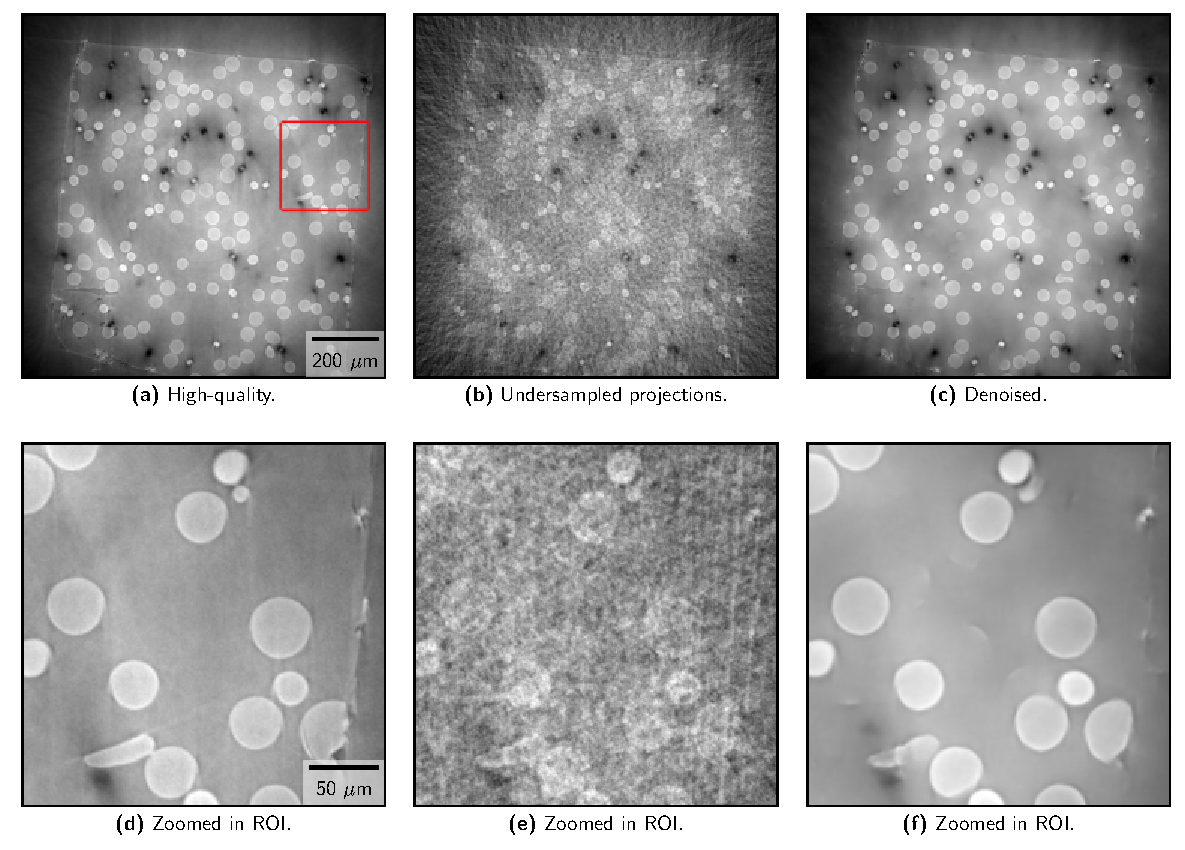
\includegraphics[width=.9\textwidth]{figures/croppeddenoising.pdf}
  \caption[Cropped image denoising]{Denoising of cropped borosilicate glass spheres dataset. Images d), e), and f) are zoomed in \gls{roi}s of images a), b), and c) respectively. The \gls{roi} is marked in a). }
  \label{fig:croppeddenoising}
\end{figure}

\begin{figure}[htbp]
  \centering
  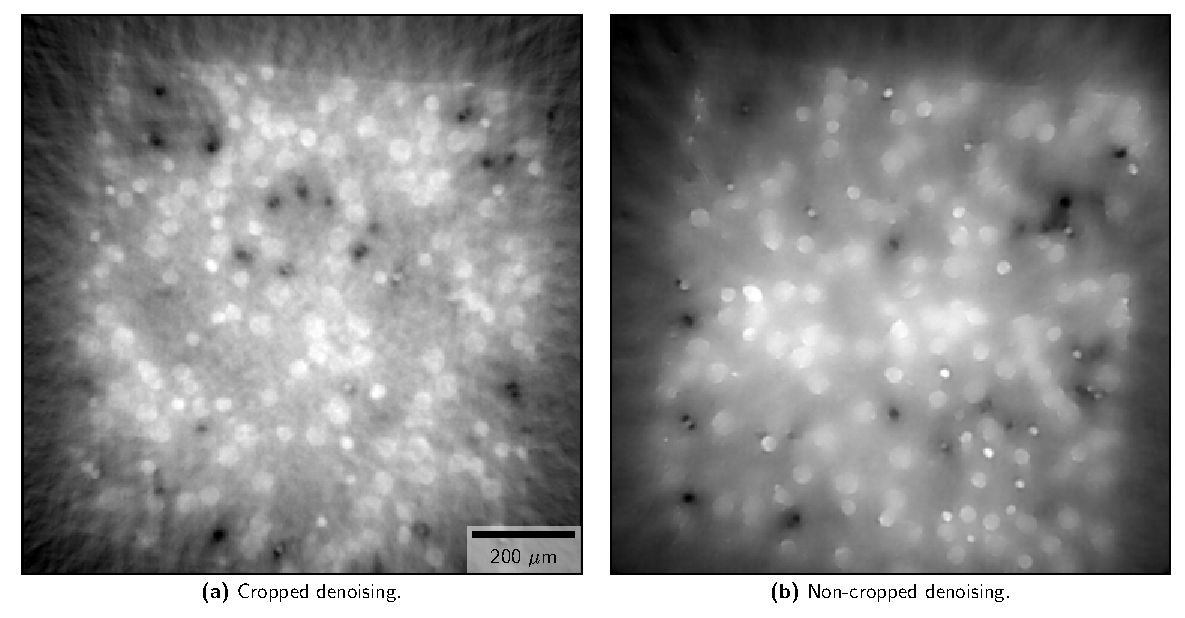
\includegraphics[width=.9\textwidth]{figures/croppednoncroppedearly.pdf}
  \caption[Non-cropped image denoising compared to non-converged cropped image denoising]{Non-cropped image denoising compared to non-converged cropped image denoising. The cropped denoising is after merely $500$ iterations of the same denoising as in \cref{fig:croppeddenoising}. The non-cropped denoising has been cropped after denoising for easier comparison. The two images are of different slices of the same dataset. }
  \label{fig:croppednoncroppedearly}
\end{figure}

\subsection{Hyperparameter and Loss Function Changes}
How the change in the loss function affected the denoising operation was explored for the dataset of the glass beads acquired from TomoBank (\cref{sec:method:datasets}). A log-cosh term (\cref{sec:ml:training:lossfunctions}) was added to the loss function, and the resulting denoised images obtained using different loss functions were compared. All other hyperparameters were kept constant, only the composition of the loss function was changed (i.e. adding log-cosh loss and reducing $\lambda_{\text{MSE}}$). The resulting two denoisings for an arbitrary slice is given in \cref{fig:losschangedenoisingcomparison}. 

While there is little visual difference in the two denoisings, the denoising containing a log-cosh based loss achieves a slight improvement in the \gls{ssim} score compared to the one without ($0.789$ vs. $0.788$). There is also no measurable difference in the training time of the network when incorporating another loss function. Because of this minor improvement with no discernable drawback, the loss function containing a log-cosh component is chosen as the default loss function for denoising in this thesis. It is possible that a larger improvement may be achievable by further tuning the weights of the different loss functions, as this has not been thoroughly explored. 

\begin{figure}[htbp]
  \centering
  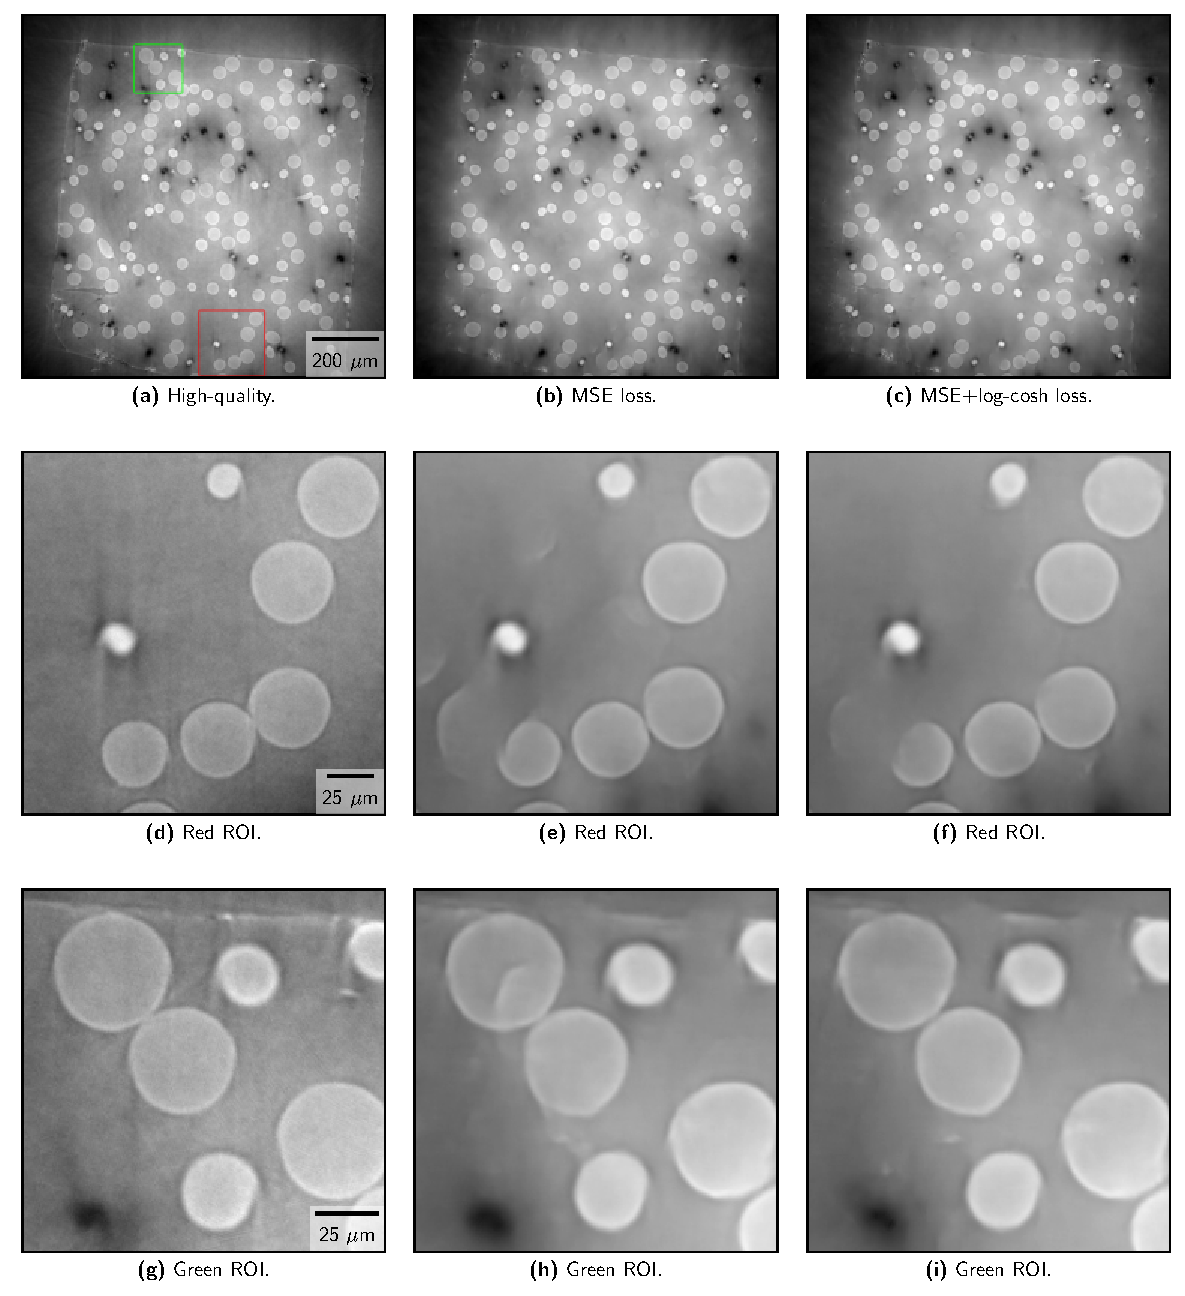
\includegraphics[width=.9\textwidth]{figures/losschangedenoisingcomparison.pdf}
  \caption[Effect on denoising of changing loss function]{Effect on denoising of changing loss function. Both denoisings are of the borosilicate glass spheres dataset with a subsampling factor of 32. Two \gls{roi}s have been marked in \textbf{(a)}, and can be seen in \textbf{(d)}-\textbf{(i)}. }
  \label{fig:losschangedenoisingcomparison}
\end{figure}

\subsection{Loss Function Evolution}
To try and understand how the TomoGAN network is performing during training, the evolution of the loss function and its components was plotted. This is given in \cref{fig:losstomo00058noadv}. We see that the main reduction in the loss of the network happens during early stages of training, especially the first few iterations. In the first $500$ iterations the loss changes from $\approx 7000$ to $\approx 100$, however a denoising after $500$ iterations does not perform well (as is given in \cref{fig:croppednoncroppedearly}a). At $100000$ iterations, the loss is $\approx 70$. In the early iterations the denoising solves for low spatial-frequency features which result in large decreases in the loss function. In later iterations high frequency information is captured, which has a smaller impact on the loss as these are finer details. 

If denoising performance could be gauged based solely on \cref{fig:losstomo00058noadv}, the denoised image after $20000$ iterations should be very similar to after $100000$ iterations. Looking at \cref{fig:iterationdenoisingcomparison} it is evident that this is not correct. The denoising after $20000$ iterations achieves an \gls{ssim} of $0.778$ compared to $0.789$ after $100000$ iterations. After $20000$ iterations, the spheres in the borosilicate glass spheres dataset are less sharp and more artefacts have been introduced. This is consistent with high frequency information being captured at later iterations. How the \gls{ssim} and \gls{mse} of an arbitrary slice of the dataset evolve through training is given in \cref{fig:ssimmseevolution}.

\begin{figure}[htbp]
  \centering
  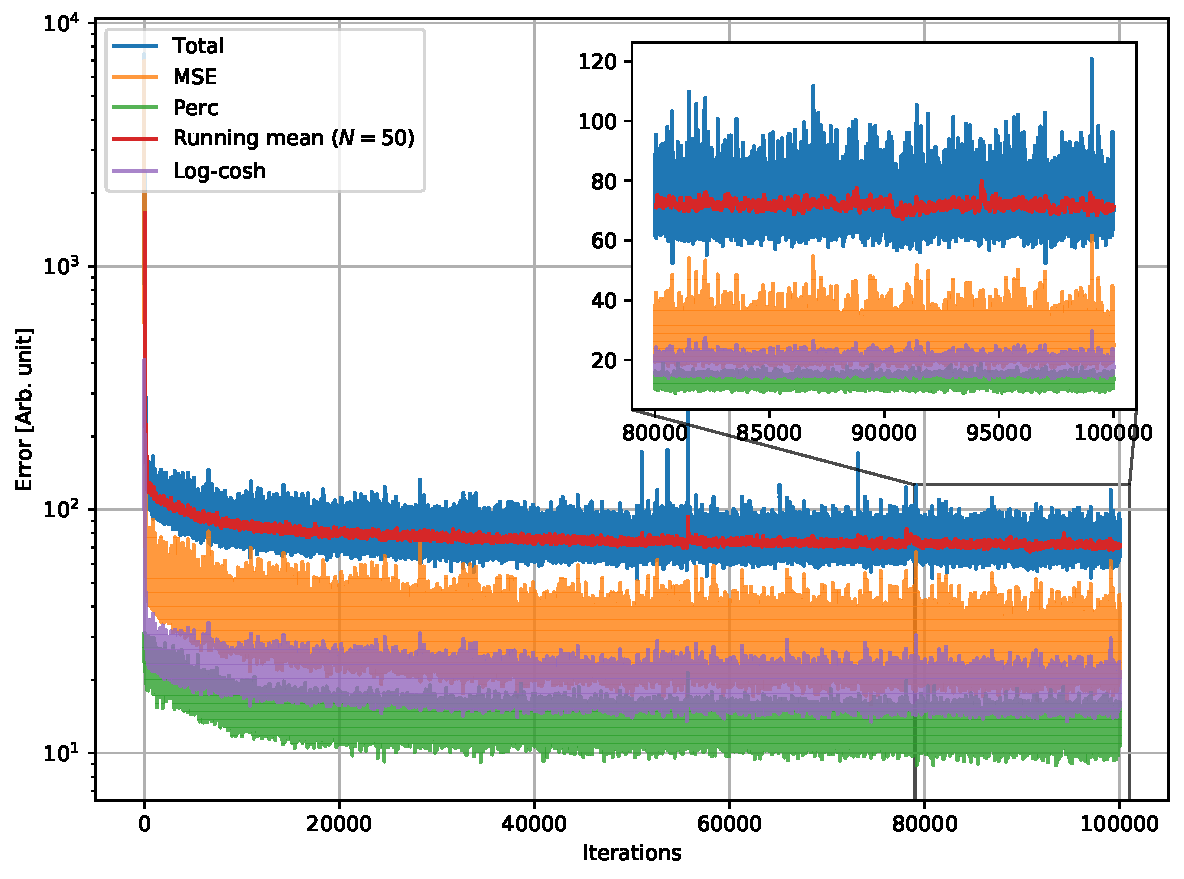
\includegraphics[width=.85\textwidth]{figures/losstomo00058ns32itd4mse035logcosh3depth1.pdf}
  \caption[Loss function evolution during training]{Plot showing how the loss function evolves during $100000$ iterations of training on the borosilicate glass spheres dataset with a subsampling factor of 32. The adversarial loss has been omitted from the plot. The inset axis shows the final $20000$ iterations. Note that the main axis is logarithmic, with the inset axis being linear. The unit of the loss is arbitrary. The running mean is the mean of the previous $50$ values. }
  \label{fig:losstomo00058noadv}
\end{figure}

\begin{figure}[htbp]
  \centering
  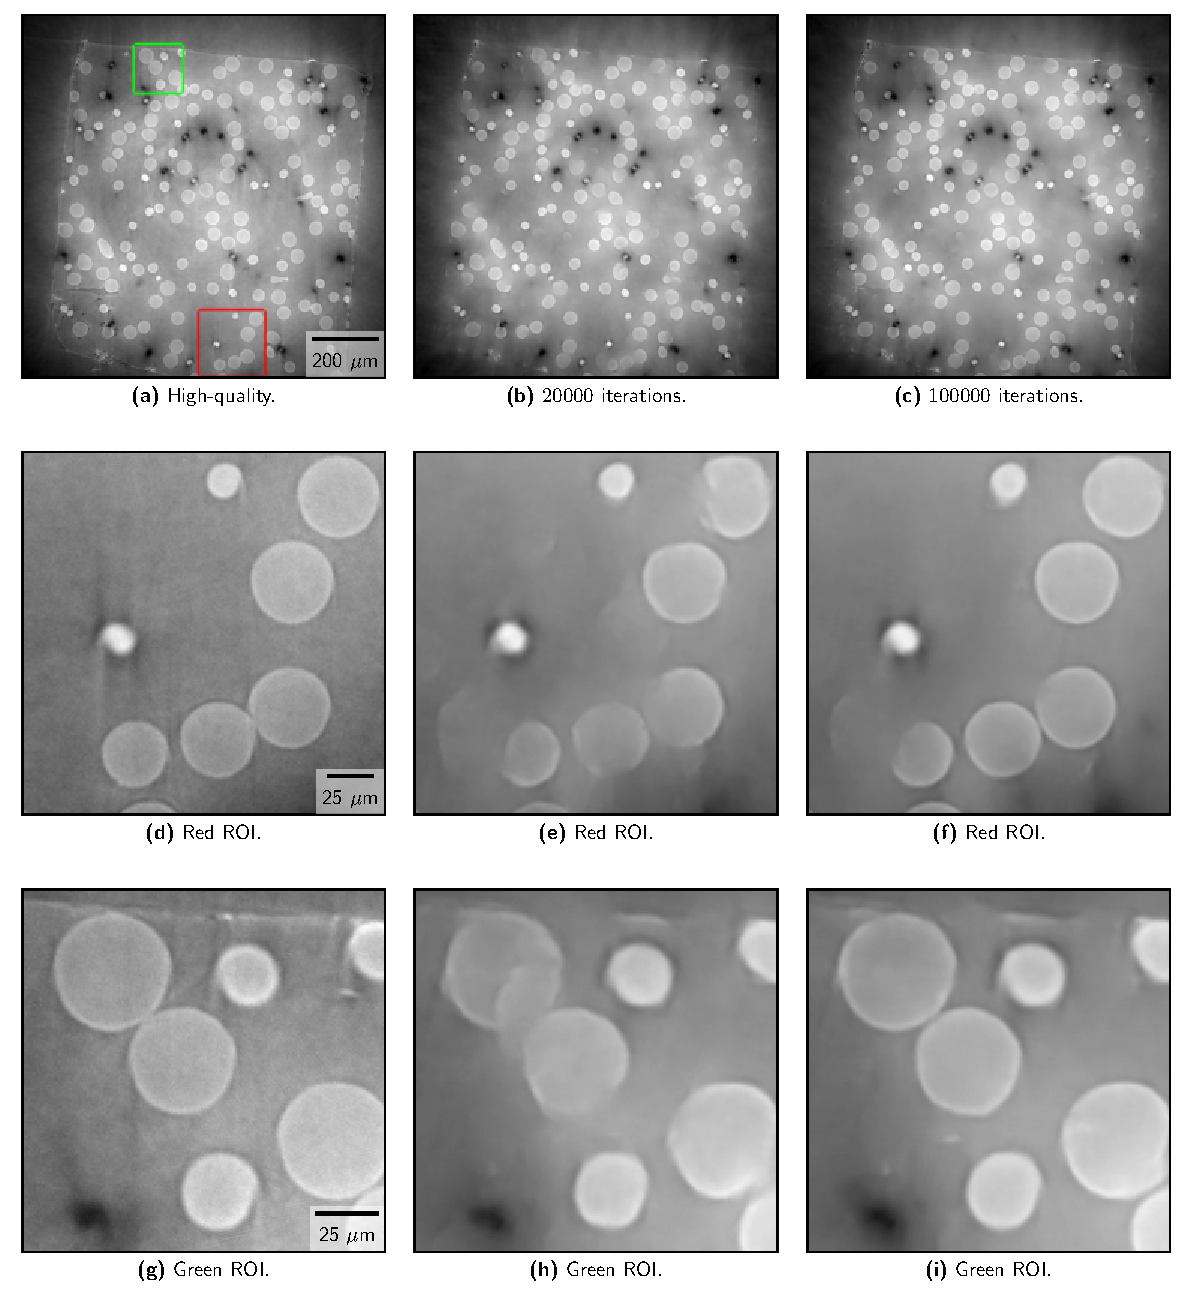
\includegraphics[width=.85\textwidth]{figures/iterationdenoisingcomparison.pdf}
  \caption[Effect on denoising of number of iterations]{Effect on denoising of number of iterations. Both denoisings are of the borosilicate glass spheres dataset with a subsampling factor of 32. Two \gls{roi}s have been marked in \textbf{(a)}, and can be seen in \textbf{(d)}-\textbf{(i)}. The scale bar for \textbf{(a)} applies to \textbf{(b)} and \textbf{(c)}, the scale bar for \textbf{(d)} applies to \textbf{(e)} and \textbf{(f)}, and the scale bar for \textbf{(g)} applies to \textbf{(h)} and \textbf{(i)}. }
  \label{fig:iterationdenoisingcomparison}
\end{figure}

\begin{figure}[htbp]
  \centering
  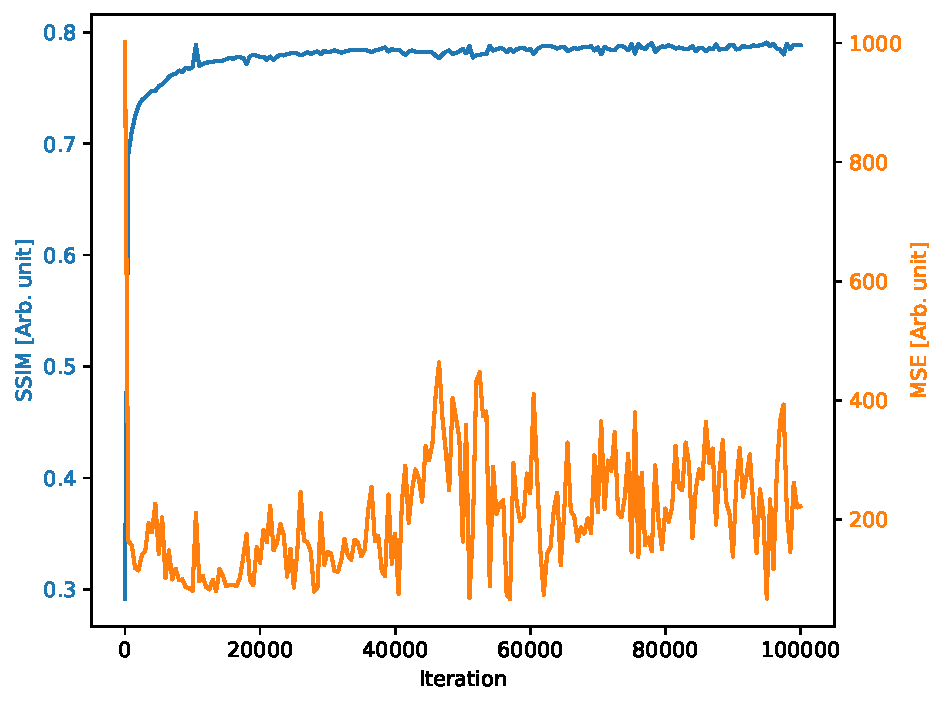
\includegraphics[width=.85\textwidth]{figures/ssimns32logcosh.pdf}
  \caption[SSIM and MSE evolution during training]{Plot showing how the \gls{ssim} and \gls{mse} of an arbitrary slice evolve during $100000$ iterations of training on the borosilicate glass spheres dataset with a subsampling factor of 32. }
  \label{fig:ssimmseevolution}
\end{figure}

\section{Soda Lime Glass Spheres}
The in-house captured dataset \gls{ihlq} (see \cref{sec:method:datasets:inhouse}) has been denoised using TomoGAN. The network has been trained to try and map the \gls{ihlq} dataset to the \gls{ihhq} dataset. As a comparison, two different reconstruction methods for the \gls{ihlq} dataset have been included: the \gls{fdk} direct reconstruction method and the \gls{piccs} iterative reconstruction method. 

\subsection{TomoGAN Compared to PICCS}
\todo[inline]{Clear boundaries, segmentation}
\todo[inline]{Compare with PICCS}
\cref{fig:kimrobertline,fig:kimroberthist}. 

\begin{figure}[htbp]
  \centering
  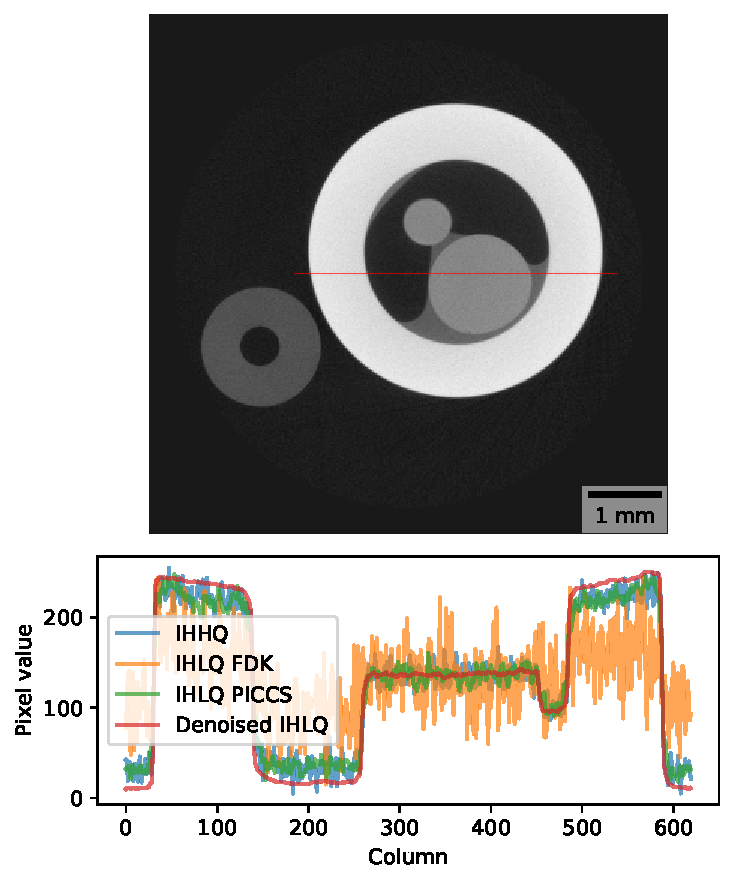
\includegraphics[width=.85\textwidth]{figures/kimrobertline.pdf}
  \caption[Pixel value plot of IHHQ and IHLQ, noisy and denoised]{The plot shows pixel values for 620 pixels on a horizontal line, as shown by the red line on the \gls{hq} image above, on the \gls{ihhq} and \gls{ihlq} dataset, both noisy and denoised. The denoised values are from denoising the \gls{ihlq} \gls{fdk} reconstruction with TomoGAN using a loss function containing \gls{mse}, log-cosh, VGG, and adversarial loss components, a depth of 1, and the network was trained for $100 000$ iterations with a mini batch size of 16. }
  \label{fig:kimrobertline}
\end{figure}

\begin{figure}[htbp]
  \centering
  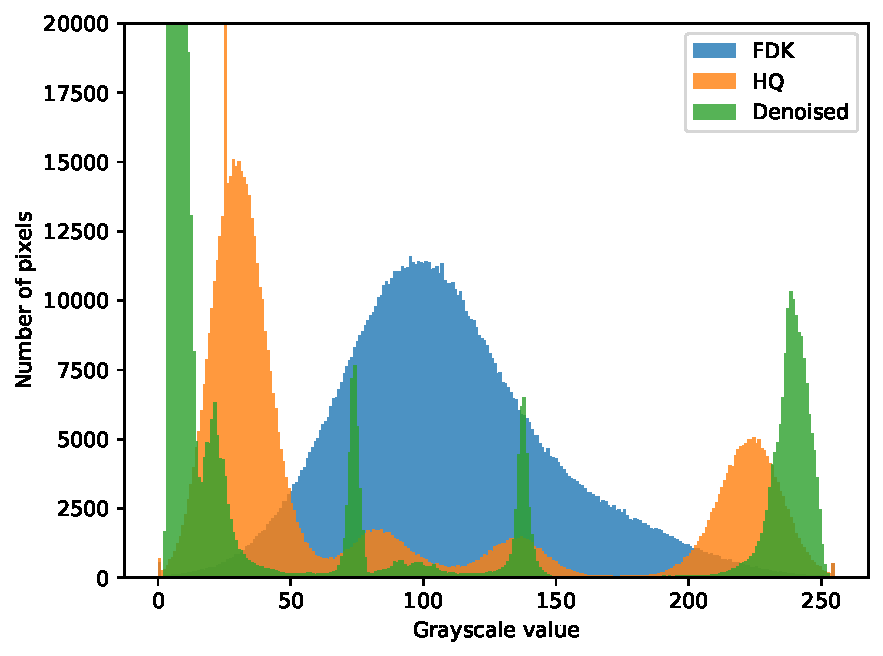
\includegraphics[width=.85\textwidth]{figures/kimroberthist.pdf}
  \caption[Histograms of IHHQ and IHLQ, noisy and denoised]{Histograms of an arbitrary slice from the \gls{ihhq} and \gls{ihlq} \gls{fdk} dataset, both noisy and denoised. The denoising was done with TomoGAN using a loss function containing \gls{mse}, log-cosh, VGG, and adversarial loss components, a depth of 1, and the network was trained for $100 000$ iterations with a mini batch size of 16. Note that the ordinate has been cropped to a max value of $20000$. }
  \label{fig:kimroberthist}
\end{figure}


\subsection{Effect of Depth Parameter on 3D Denoising}
For this dataset, the 3D stability of the denoising method has been explored. Because the TomoGAN network uses 2D convolutions (see \cref{sec:method:tomogan}), it is primarily a 2D denoising method. The network allows for 3D information to be included in the denoising by adjusting a depth parameter, which looks at adjacent slices and performs a $1\times1$ convolution across them, however by inspecting the structure of the network (see \cref{fig:tomoganstructure}) it is evident that this 3D information is only used at early stages of the denoising. Only the initial $1\times1$ convolutional layer, before the down sampling part of the network, looks at the depth. 

The result of the limited use of 3D information is that the network has a plane that is the primary focus of the denoising. By inspecting \cref{fig:bigfigure} it is evident that the denoising is done on the axial plane. For a denoising with a depth of 1, it is very clear that there is a lack of consistency between axial planes. Looking at the yellow \gls{roi} there is banding artefacts introduced between the axial layers. The same denoising with a depth of 7 still contains some of this banding artefacting, however the introduction of some 3D knowledge reduces the artefacting. When instead looking at the blue \gls{roi}, which is of the axial plane, there is no such banding artefacts. By visual inspection we see that the banding artefacting is reduced when the depth is increased. The specific depth that yields the best results is dependent on dataset characteristics, such as feature resolution \cite{liu2020tomogan}. 

In the green \gls{roi} in \cref{fig:bigfigure} we see details that were indiscernible in the low-quality \gls{ihlq} \gls{fdk} reconstruction, and not properly visible in the \gls{ihlq} \gls{piccs} reconstruction, are captured by TomoGAN. These details are clearly visible even when only a depth of 1 is used, however they are highly prone to banding artefacts between layers, and increasing the depth helps on this. 

\begin{figure}[htbp]
  \centering
  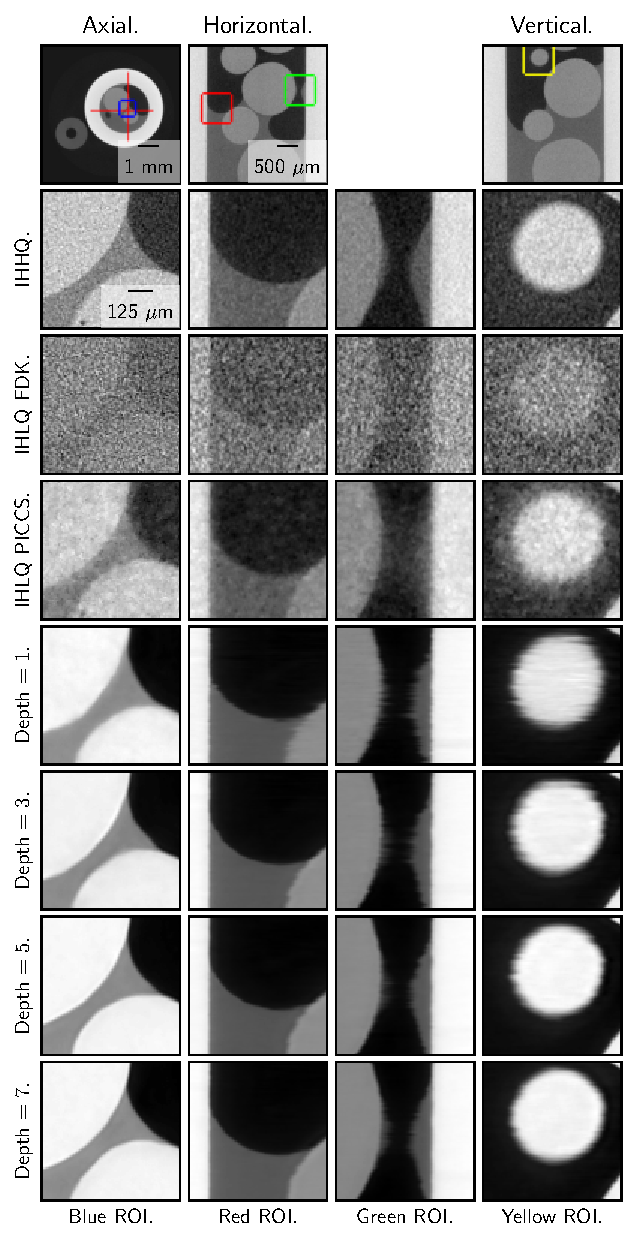
\includegraphics[width=.77\textwidth]{figures/bigfigure.pdf}
  \caption[Different reconstructions and denoisings of the IHLQ and IHHQ datasets]{Different reconstructions and denoisings of the \gls{ihhq} and \gls{ihlq} datasets. The top three images are full views of the \gls{ihhq} dataset. The red horizontal line in the top left figure corresponds to the sagittal view in the top middle figure, and the red vertical line corresponds to the coronal view in the top right figure. Four \glspl{roi} have been marked in the top figures and have been zoomed in for the different reconstructions and denoisings. All zoomed in figures have the same scale bar. }
  \label{fig:bigfigure}
\end{figure}




\section{Pierre Shale}
\subsection{Denoising Without High-quality Dataset}
\todo[inline]{Shows limitations of method: requires a high-quality similar dataset (i.e. some ground truth) to work properly. Any given trained network doesn't work for all other dataset. }
\cref{fig:shale}

\begin{figure}
  \begin{subfigure}[t]{\textwidth}
    \centering
    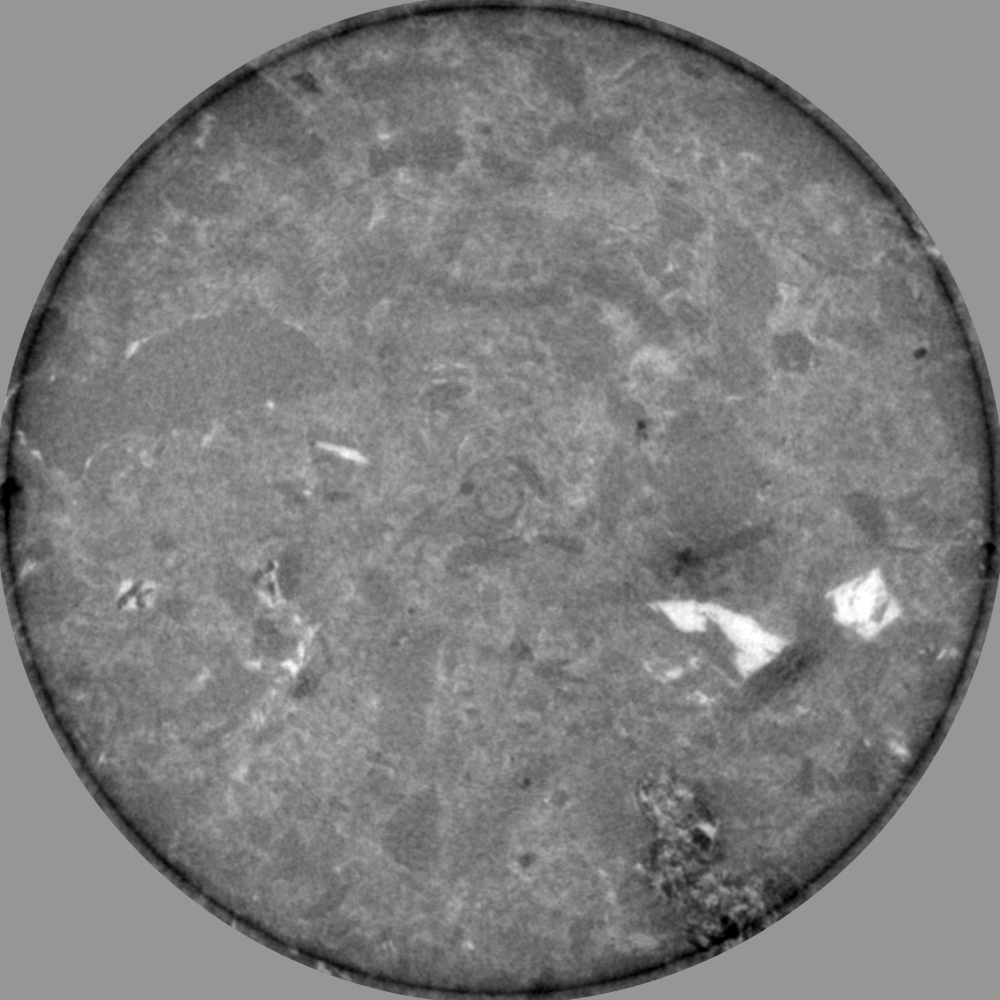
\includegraphics[width=.45\textwidth]{figures/shale/shale_ns/0.png}
    \caption{Original image. }
  \end{subfigure}

  \medskip

  \begin{subfigure}[t]{.45\textwidth}
    \centering
    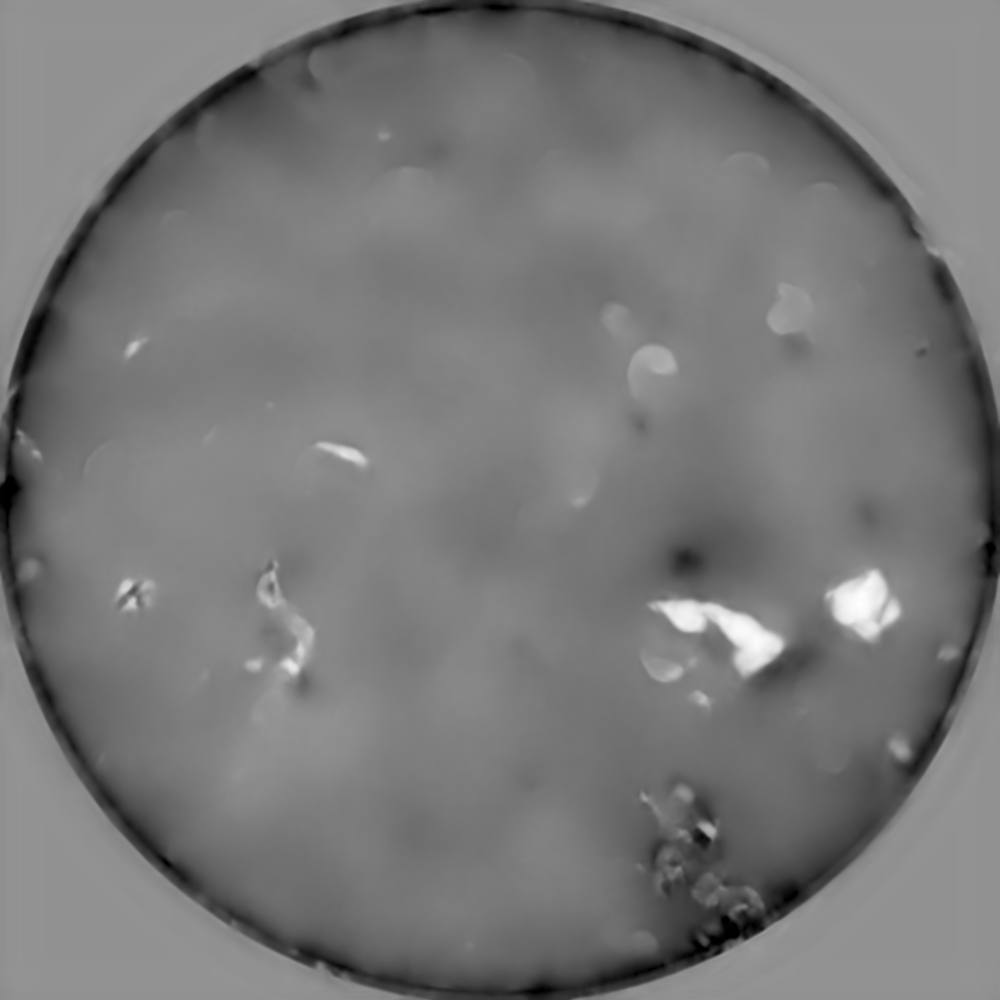
\includegraphics[width=\linewidth]{figures/shale/shale_dn_tomo00058/0.png}
    \caption{tomo\_00058. }
  \end{subfigure}
  \hfill
  \begin{subfigure}[t]{.45\textwidth}
    \centering
    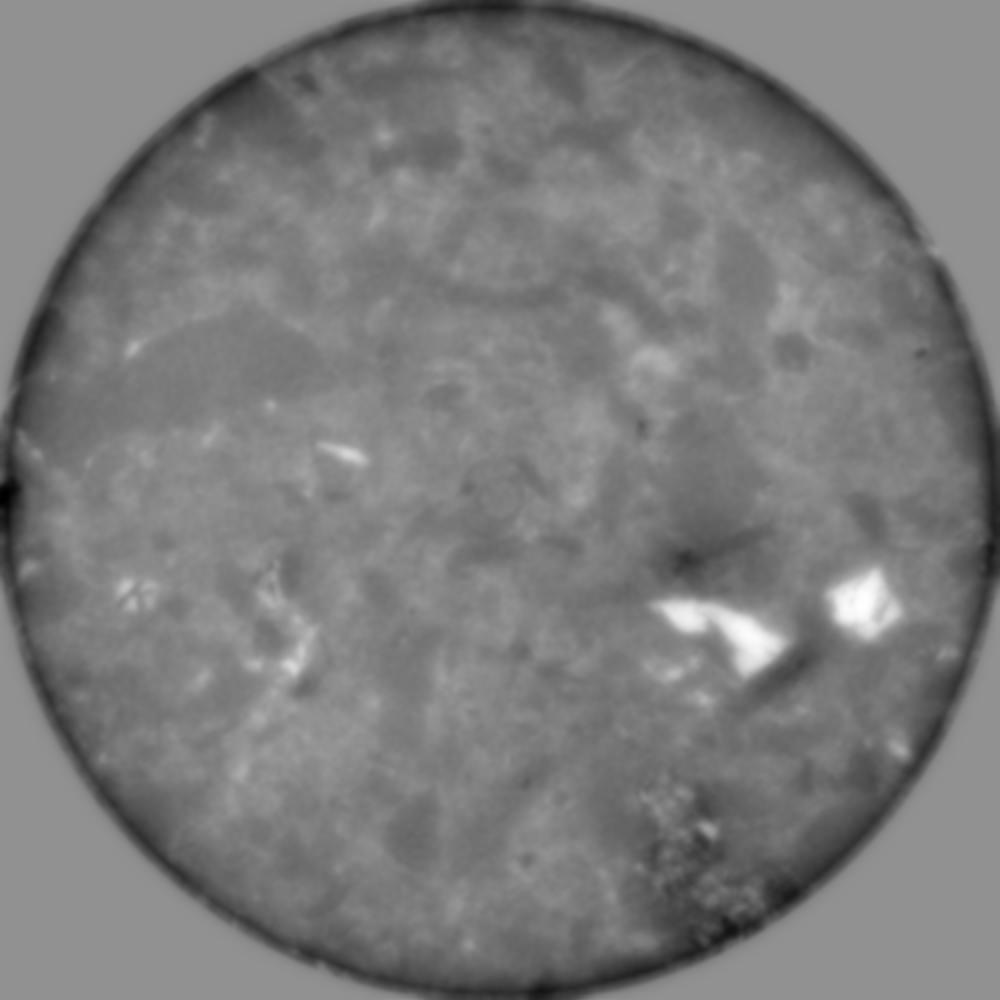
\includegraphics[width=\linewidth]{figures/shale/shale_dn_tomo00001/0.png}
    \caption{tomo\_00001. }
  \end{subfigure}

  \medskip

  \begin{subfigure}[t]{.45\textwidth}
    \centering
    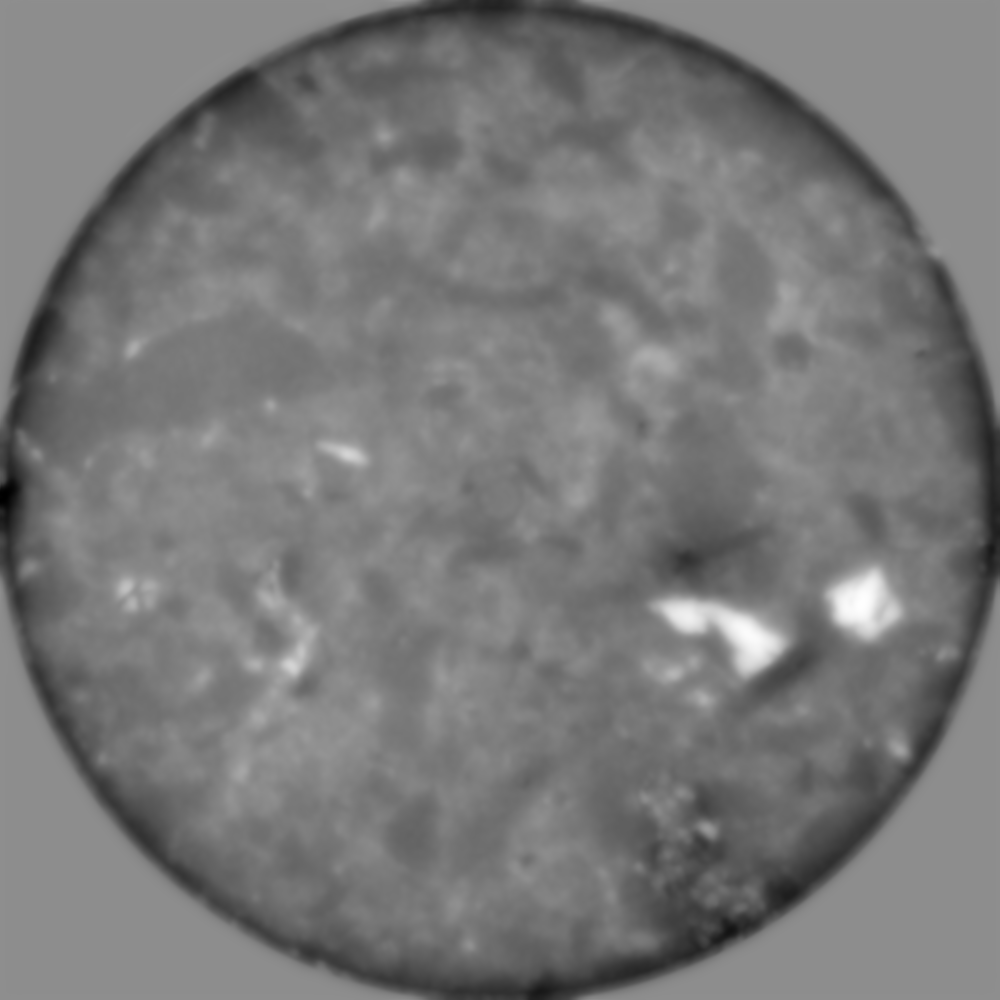
\includegraphics[width=\linewidth]{figures/shale/shale_dn_tomo00002/0.png}
    \caption{tomo\_00002. }
  \end{subfigure}
  \hfill
  \begin{subfigure}[t]{.45\textwidth}
    \centering
    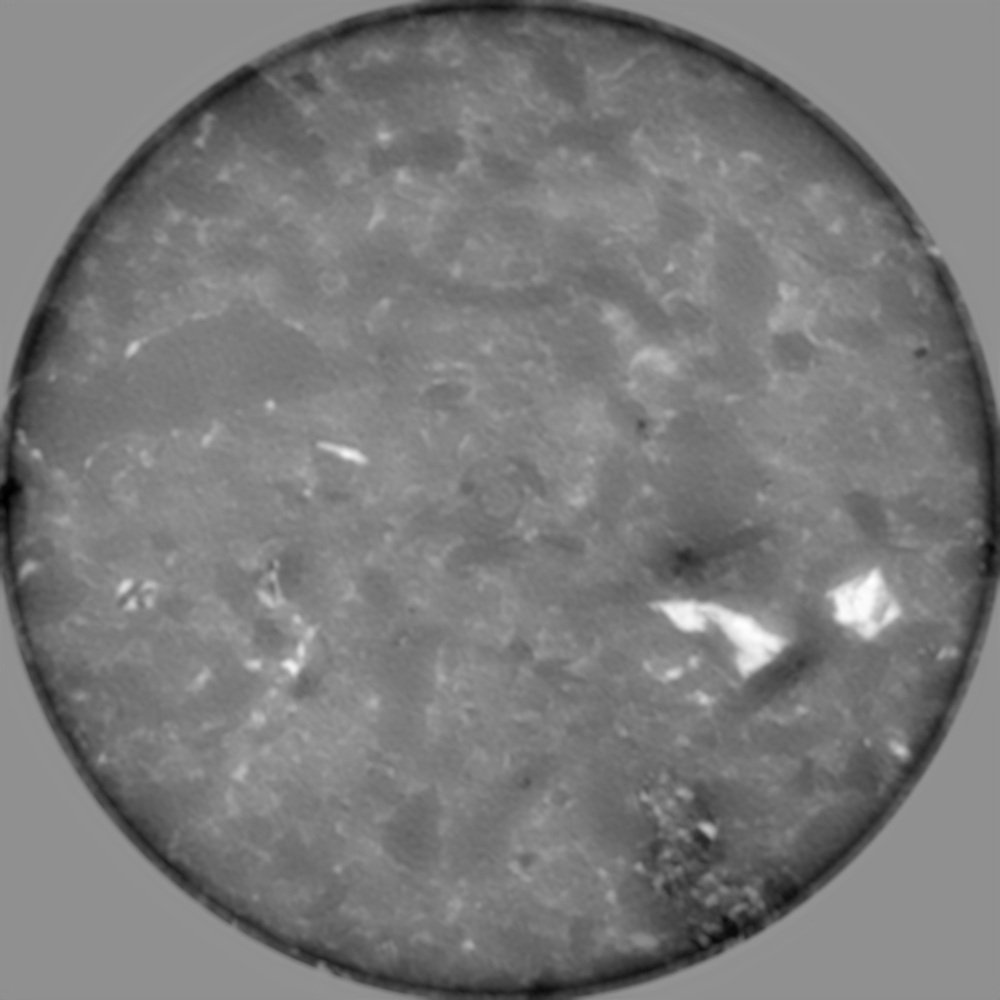
\includegraphics[width=\linewidth]{figures/shale/shale_dn_tomo00002min7/0.png}
    \caption{tomo\_00002min7. }
  \end{subfigure}
  \caption[Attempted shale denoising]{Attempted shale denoising. }
  \label{fig:shale}
\end{figure}




%Plot types: 
%\begin{itemize}
%    \item \gls{ssim} and \gls{mse} changes during training.
%    \item Loss function evolution.
%    \item Line plot of gt, ns, and different loss functions?
%    \item Histograms of gt, ns, denoised
%    \item Zoomed in region of interest.
%    \item Axial, sagittal, and coronal plots of (at least Kim Robert's dataset) different depth parameters.
%    \item Compare denoising of different subsamplings (8, 16, 32, 48)
%    \item Activation plot of network layers.
%\end{itemize}